\chapter[面向车载信息物理融合的通信与计算资源协同优化关键技术]{面向车载信息物理融合的通信与计算资源协同优化\\关键技术}
本章将研究面向车载信息物理融合的通信与计算资源协同优化关键技术。
本章内容安排如下:
\ref{section 3-1} 节是本章的引言,介绍车联网中资源分配与任务卸载研究现状、目前研究的不足,以及本章的主要贡献。
\ref{section 3-2} 节阐述了协同通信与计算卸载场景。
\ref{section 3-3} 节形式化定义了协同资源优化问题。
\ref{section 3-4} 节设计了一种基于博弈理论多智能深度强化学习的资源优化策略。
\ref{section 3-5} 节搭建了仿真实验环境并进行了性能验证。
\ref{section 3-6} 节总结本章的研究工作。

\section{引言}\label{section 3-1}

车联网的最新进展为新兴的智能交通系统的发展铺平了道路,例如协同自主驾驶\cite{bagheri20215g}和车载信息物理融合系统\cite{mugabarigira2023context}。
然而,实现车载信息物理融合系统需要大量的数据传输和密集的任务计算。
例如,现代汽车(如特斯拉Model X)已配备了8个摄像头、12个超声波雷达和1个毫米波雷达,其极大增加了感知数据计算的需求。
另一方面,车联网中有限的通信和计算资源使得支持实时 VCPS 构建充满挑战。
因此,研究 VCPS 中高效的实时任务卸载和异构资源分配是当务之急。

车载边缘计算\cite{lang2022cooperative}作为一种有前途的范式出现,以促进车联网边缘的任务处理。
研究人员为VEC的发展付出了巨大的努力 \cite{liu2021fog, dai2021edge, zhang2022digital, liu2020adaptive, liu2018coding},其中边缘节点(如5G基站和路侧设备)搭载计算单元,可以处理车辆通过 V2I 通信上传的数据处理任务。
然而,上述研究都没有利用非正交多址\cite{islam2017power}技术来提高网络容量。
部分研究在车联网中考虑了NOMA\cite{patel2021performance, zhang2021centralized, zhu2021decentralized, liu2019energy},其中车辆可以利用相同频率的频谱资源以不同的传输功率与边缘节点进行通信。
然而,这些研究只考虑了单个边缘节点的情况,不能处理不同边缘节点之间的干扰。
为了提高系统的可靠性,部分研究设计了通信和计算资源的分配机制,以抵消VEC中V2I信道条件和动态可用计算资源的时变影响\cite{liu2021rtds, liu2022a, chen2020robust, liu2014temporal, liu2016cooperative}。
然而,上述研究工作都没有研究实时任务卸载和通信/计算资源分配的协同效应。
一些研究通过整合任务卸载和资源分配制定了联合优化模型 \cite{dai2021asynchronous, dai2022a},但这些研究主要基于集中式调度,这可能会阻碍车联网系统可扩展性。
为解决这个问题,多智能体深度强化学习\cite{kumar2022multi}被提出用于车联网资源优化 \cite{alam2022multi, zhang2021adaptive, nie2021semi}。
另一方面,部分研究结合了强化学习和博弈论 \cite{zheng2022stackelberg, albaba2021driver, rajeswaran2020a}来解决复杂的优化问题。
然而,这些解决方案都不能直接应用于车联网中联合实时任务卸载和异构资源分配。

本章提出了一种基于博弈理论的多智能体深度强化学习的联合任务卸载和资源分配的分布式调度方案。
特别地,本章首先将任务卸载决策过程建模为一个严格势博弈(Exact Potential Game, EPG)\cite{chew2016potential}模型,并证明其在所设计的势函数下具有纳什均衡(Nash Equilibrium, NE)存在性和收敛性。
在该博弈中,边缘节点是理性的玩家,其目标为实现自身利益最大化(最大化实时任务的服务率,即在任务截止时间前完成的任务数占总任务数的比率)。
根据势博弈理论,NE可以基于所设计的势函数最大化每个边缘节点的势来实现。
因此,势博弈中的势函数适合作为所提多智能体分布式深度确定性策略梯度(Multi-Agent Distributed Distributional Deep Deterministic Policy Gradient, MAGT)算法中边缘节点的奖励函数。
然后,本章将资源分配问题分为两个独立的凸优化问题,并提出了一个基于梯度的迭代方法和卡罗需-库恩-塔克(Karush-Kuhn-Tucher, KKT)条件的最优解。

本章对 VCPS 中实时任务卸载和异构资源分配进行了联合研究并解决以下挑战。
首先,V2I上行链路受到使用相同信道的车辆干扰的影响,其影响取决于边缘节点分配的传输功率。
其次,由于计算密集型和延迟敏感型任务的时变分布,不同边缘节点之间的工作负载分配严重失衡。
再次,让边缘节点仅凭其本地知识就能独立有效地决定任务卸载和资源分配的决策是具有挑战性的。
因此,研究联合实时任务卸载和异构资源分配的有效和分布式方法是当务之急,但也具有挑战性。

基于以上分析,本章致力于研究基于NOMA的车载边缘计算中协同资源优化问题,并提出有效分布式算法进行实时任务卸载和异构资源分配。
本章的主要贡献概述如下:
第一,提出了一个基于NOMA的VEC架构,车辆共享相同频率的带宽资源与边缘节点通信,边缘节点为其分配不同的传输功率。
车辆请求具有不同计算资源需求和完成期限的计算任务,其可通过V2I通信上传到边缘节点进行进一步计算。
边缘节点具有异质计算能力,即CPU时钟频率,并选择分配计算资源在本地执行任务,或者通过有线连接将任务迁移到邻近的边缘节点处理。
第二,提出了一个协同资源优化(Cooperative Resource Optimization, CRO)问题,该问题联合卸载任务并分配通信和计算资源以最大化服务率。
具体地,建立了一个V2I传输模型,其中边缘内和边缘间的干扰都是基于NOMA原则来建模的。
然后,通过考虑异构边缘节点的合作,建立了一个任务卸载模型。
第三,提出了基于博弈模型的多智能体深度强化学习来优化通信与计算资源。
具体地,将CRO分解为两个子问题,即任务卸载和资源分配。
将任务卸载子问题建模为边缘节点之间的非合作博弈,并进一步证明其为具有NE存在和收敛性的EPG。
然后,设计了一种MAGT算法,其为D4PG\cite{barth2018distributed}的多智能体版本,以实现纳什均衡,其中边缘节点作为独立的智能体,通过采用实现势作为奖励来评估任务卸载的动作。
此外,将资源分配子问题划分为两个独立的凸问题,并分别通过基于梯度的迭代方法和KKT条件得出最优解。
第四,基于现实世界的车辆轨迹建立了仿真模型,并介绍了除主要指标外的四个指标,包括平均处理时间(Average Processing Time, APT)、平均服务时间(Average Service Time, AST)、平均实现势(Average Achieved Potential, AAP)和本地处理与迁移的比例(Proportion of Locally Processing to Migration, PLPM)。
并实现了所提算法,以及四种有竞争力的解决方案,分别是最优资源分配和任务全迁移(Optimal Resource Allocation and Task Migration Only, ORM)、最优资源分配和任务仅本地处理(Optimal Resource Allocation and Task Local Processing Only, ORL)、分布式深度确定性策略梯度(Distributed Distributional Deterministic Policy Gradient, D4PG)\cite{barth2018distributed},以及多智能体深度确定性策略梯度\cite{zhang2021adaptive},并通过仿真结果证明了所提算法的优越性。

\section{协同通信与计算卸载场景}\label{section 3-2}

本章提出了一个协同通信与计算卸载场景,如图\ref{fig 3-1}所示,沿路安装的基础设施包括5G基站和RSU(如$e_1$$\sim$$e_3$)都安装了不同的计算单元(即CPU芯片),其可作为边缘节点以加速移动车辆卸载的计算任务。
任务随机地到达车辆,其中不同任务可能包含不同的待计算数据。
车辆可以在通信范围内通过V2I通信与边缘节点进行通信。
然后,车辆将任务上传到附近的边缘节点,传输功率由相应的边缘节点分配。
通过在车辆上采用叠加编码(Superposition Coding, SC)技术和在边缘节点上采用串行干扰消除(Successive Interference Cancellation, SIC)\cite{khan2021noma}技术,车辆可以共享同一频率的带宽资源。
在基于NOMA的VEC中,在对弱信号车辆的信号进行解码之前,先由边缘节点对强信号车辆的信号进行解码和消除。
此外,边缘节点之间通过一个有线网络连接。
边缘节点可以决定是否在本地执行收到的任务或通过有线连接将其迁移到其他边缘节点。
最后,边缘节点为需要处理的任务分配计算资源。

\begin{figure}[h]
\centering
  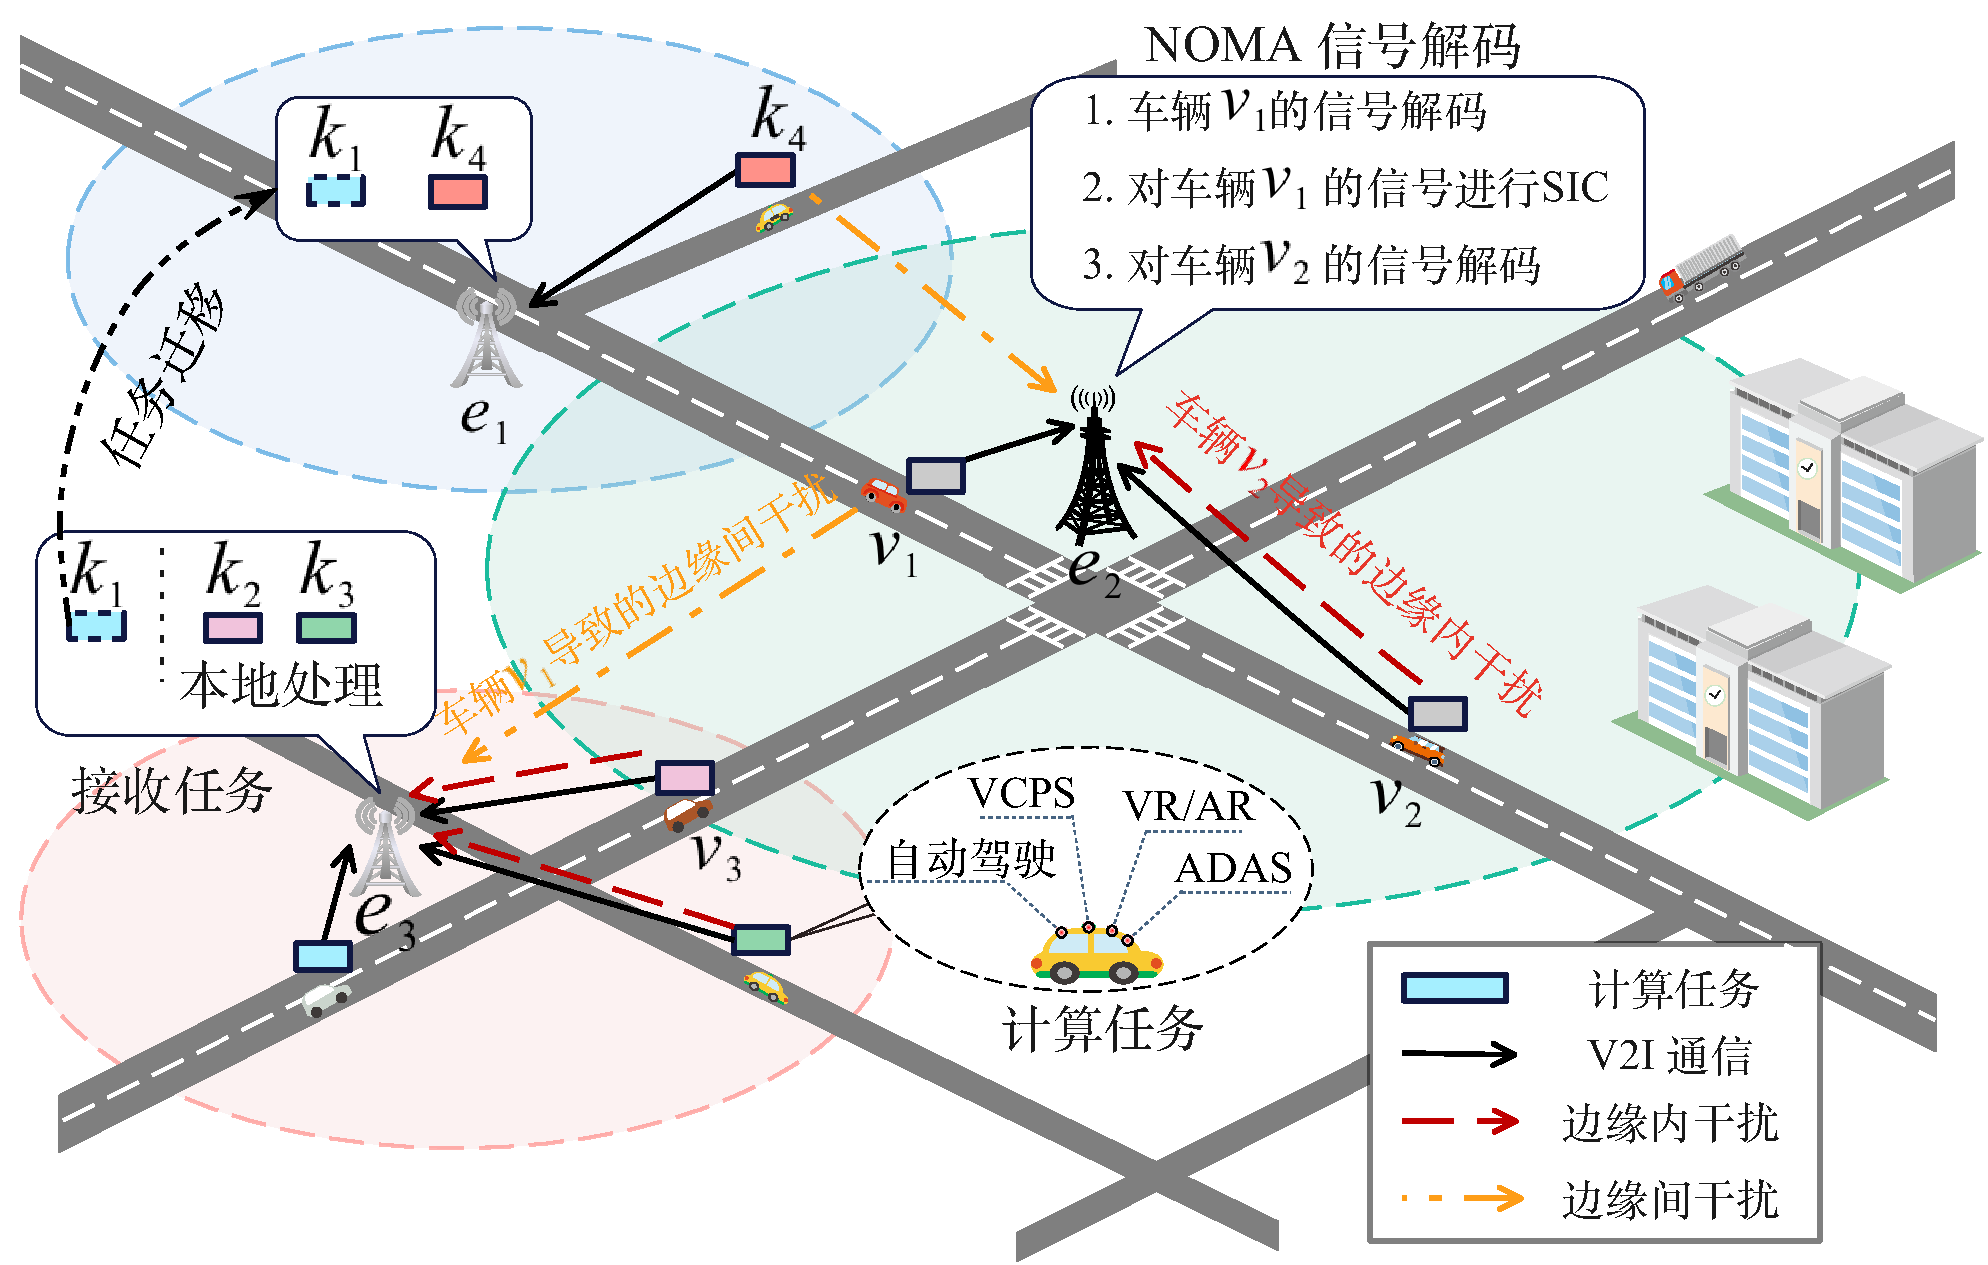
\includegraphics[width=1\columnwidth]{Fig3-1-noma-architecture.pdf}
  \bicaption{协同通信与计算卸载场景}{Cooperative transmission and computation offloading scenario}
  \label{fig 3-1}
\end{figure} 

本系统的特点总结如下:
首先,车辆请求的计算任务可能有不同的数据大小、计算资源要求和截止时间。
因此,任务完成情况(即任务是否能在最后期限前成功完成)当被卸载到具有不同计算能力(即CPU时钟频率)的边缘节点时可能有所不同。
其次,增加车辆的传输功率虽然可能会提高V2I传输率,但是也会由于边缘内和边缘间的干扰增强而损害其他V2I上行链路。
此外,边缘节点的功率分配随着时间的推移而变化,并且相互之间是未知的。
因此,边缘节点必须通过考虑其他边缘节点的功率分配的影响来确定车辆的传输功率。
最后,由于任务的随机到达和车辆的时变分布,边缘节点的工作负载可能不平衡。
当一个边缘节点负担过重时,将额外的任务迁移到其他有多余计算资源的边缘节点以加快处理是合适的。
然而,通过有线连接将任务数据传输到边缘节点也会延长任务服务时间。

进一步,本章提供一个例子来更好地说明上述问题。
如图\ref{fig 3-1}所示,车辆$v_1$和$v_2$通过V2I通信上传计算任务。
由于边缘节点$e_2$和车辆$v_1$之间的V2I信道条件优于车辆$v_2$和$v_3$,车辆$v_1$的信号可以通过将其他信号视为噪声来进行优先解码。
然后,在对车辆$v_2$和$v_3$的信号进行解码时,车辆$v_1$的信号可以被边缘节点$e_2$通过SIC进行消除。
然而,车辆$v_1$的信号在V2I传输过程中可能受到车辆$v_2$的干扰;这种干扰被称为“边缘内干扰”,因为车辆$v_1$和$v_2$处于同一个边缘节点$e_2$的无线电覆盖范围内。
另一方面,车辆$v_3$的信号可能受到车辆$v_1$的干扰,这种来自其他边缘节点的干扰被称为“边缘间干扰”。
此外,很明显,边缘节点$e_1$和$e_3$之间的任务负载是不均匀的,因为在边缘节点$e_3$中有三个任务(即$k_1$、$k_2$和$k_3$),但在边缘节点$e_1$中只有一个任务$k_4$。
假设边缘节点$e_1$的计算资源明显多于边缘节点$e_3$的资源,那么任务$k_1$应该通过有线网络迁移到边缘节点$e_1$,因而可以在更短的时间内得到服务。
如上所述,通过设计一个有效的分布式调度机制来实现实时任务卸载和异构资源分配,从而优化系统的整体性能,这对利用边缘节点之间的协作通信和计算是非常关键且具有挑战性的。

\section{协同资源优化问题定义}\label{section 3-3}

离散时间片的集合用$\mathbf{T}=\{1, \ldots, t, \ldots, T\}$表示,其中$T$是时间片的数量。
车辆的集合用$\mathbf{V}=\{1, \ldots, v, \ldots, V\}$表示,车辆$v \in \mathbf{V}$在$t$时的位置用$l_{v}^{t}$表示。
车辆$v$在时间$t$的任务到达概率用$\tau_{v}^{t}$表示,并用$\mathbf{K}_{v}$表示车辆$v$请求的任务集合。
车辆$v$在时间$t$要求的任务$k_{v}^{t} \in \mathbf{K}_{v}$由三元组表示$k_{v}^{t}=\left(d_{k}, c_{k}, t_{k}\right)$,其中$d_{k}$、$c_{k}$和$t_{k}$分别为数据大小、处理一位数据的CPU周期和任务处理截止时间。
边缘节点的集合用$\mathbf{E}=\{1, \ldots, e, \ldots, E\}$表示,边缘节点$e \in \mathbf{E}$由四元组$e=\left(p_{e}, c_{e}, g_{e}, l_{e}\right)$表示,其中$p_{e}$是V2I通信的最大功率,$c_{e}$是计算频率,$g_e$是V2I通信范围,$l_{e}$是位置。
边缘节点之间有线通信的传输速率用$z$表示。
车辆$v$与边缘节点$e$在时间$t$的距离用$\operatorname{dis}_{v, e}^{t}$表示。
在$t$时间,在边缘节点$e$的无线电覆盖范围内的车辆集合用$\mathbf{V}_{e}^{t}=\left\{v \mid \operatorname{dis}_{v, e}^{t} \leq g_{e}, \forall v \in \mathbf{V}\right\}, \mathbf{V}_{e}^{t} \subseteq \mathbf{V}$表示。
V2I通信的带宽用$b$表示。

\begin{figure}[h]
\centering
  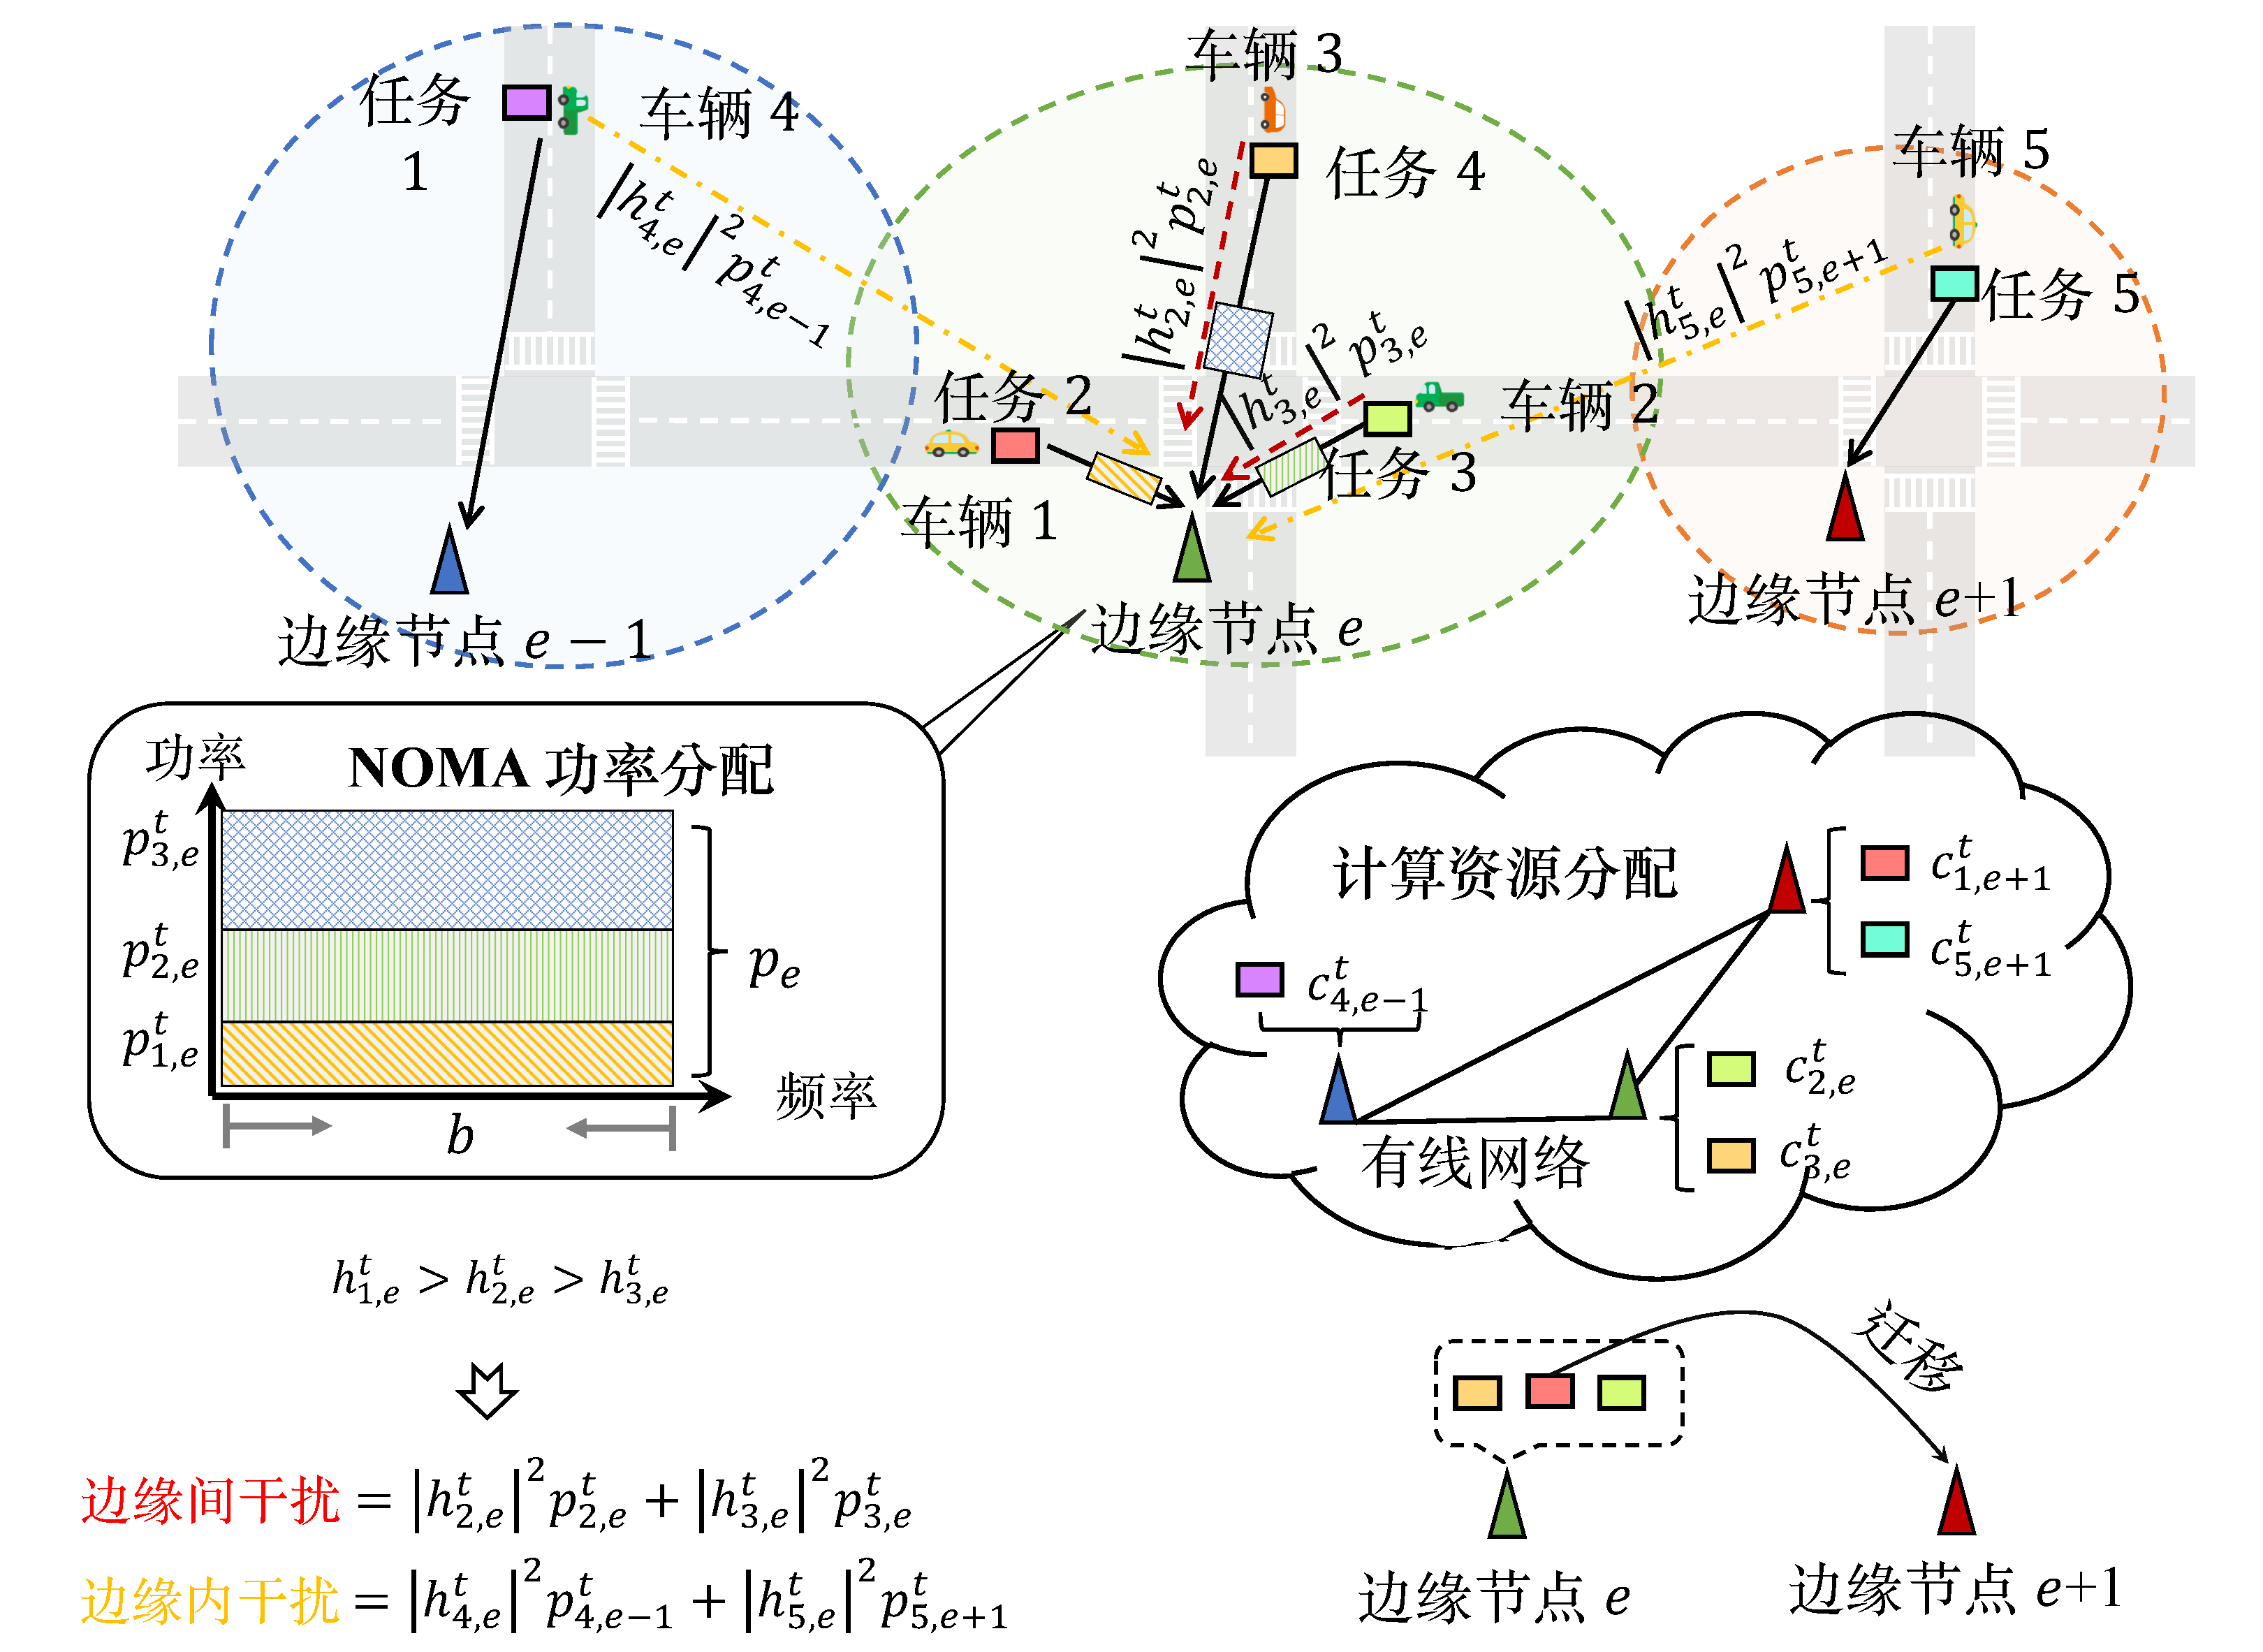
\includegraphics[width=1\columnwidth]{Fig3-2-system-model.pdf}
  \bicaption{V2I 传输与任务卸载模型}{V2I transmission and task offloading model}
  \label{fig 3-2}
\end{figure}

\subsection{V2I 传输模型}

本章节构建了V2I传输模型,如图\ref{fig 3-2}所示, 其中边缘内和边缘间干扰的干扰是基于NOMA原则建模的。
本章将边缘节点$e$在时间$t$分配的车辆$v$的传输功率表示为$p_{v, e}^{t}$。
分配的功率之和不能超过边缘节点$e$的V2I通信的最大功率,即$\sum_{\forall v \in {V}_{e}^{t}} p_{v, e}^{t} \leq p_{e}$。
然后,车辆$v$和边缘节点$e$之间在时间$t$的信道增益用$h_{v, e}^t$表示,可通过以下公式计算\cite{sun2020performance}
\begin{equation}
	h_{v, e}^t = \frac{\eta_{v, e}}{{\operatorname{dis}_{v, e}^{t}}^{\varphi/2}}
\end{equation}
\noindent 其中$\eta_{v, e}$是瑞利分布的小尺度衰减,即$\eta_{v, e} \sim \mathcal{CN}(0, 1)$,$\varphi$是大尺度路径损耗指数。
因此,比车辆$v$的瞬时信道条件更差的车辆集合用$\mathbf{V}_{h_{v, e}}^{t}$表示,其表示为
\begin{equation}
	\mathbf{V}_{h_{v, e}}^{t} = \left \{ v^{\prime} \mid  \left|h_{v^{\prime}, e}^t \right|^{2} < \left| h_{v, e}^t\right |^{2} , \forall v^{\prime} \in \mathbf{V}_{e}^{t} \right \}
\end{equation}
在确定了每个车辆$v \in \mathbf{V}_{e}^{t}$的传输功率后,边缘节点$e$的观测信号可以表示为\cite{islam2017power}
\begin{equation}
	y_e^{t} = \sum_{\forall v \in \mathbf{V}_{e}^{t}} p_{v, e}^{t} s_{v, e}^{t} h_{v, e}^t + \sum\limits_{\forall e^{\prime} \in \mathbf{E} / \{e\}} \sum\limits_{\forall v^{\prime} \in \mathbf{V}_{e^{\prime}}^{t}} p_{v^{\prime}, e^{\prime}}^{t} s_{v^{\prime}, e^{\prime}}^{t} h_{v^{\prime}, e}^t + N_{0}
\end{equation}
其中$s_{v, e}^{t}$是用于车辆$v$的信息,$N_{0}$是AWGN。
根据NOMA原则,边缘节点$e$可以通过SIC消除信道条件比车辆$v$好的车辆的信号 \cite{du2021ji}。
因此,车辆$v$和边缘节点$e$之间在时间$t$的信号与干扰加噪声比(Signal-to-Interference-plus-Noise Ratio, SINR)用$\mathrm{SINR}_{v, e}^t$表示,可以通过以下公式计算
\begin{equation}
	\mathrm{SINR}_{v, e}^t = \frac{ |h_{v, e}^t| ^{2}  p_{v, e}^{t}}{ \underbrace{\sum\limits_{\forall v^{\prime} \in \mathbf{V}_{h_{v, e}}^{t}} |h_{v^{\prime}, e}^t|^2 p_{v^{\prime}, e}^{t}}_{\text {边缘内干扰}} + \underbrace{\sum\limits_{\forall e^{\prime} \in \mathbf{E} / \{e\}} \sum\limits_{\forall v^{\prime} \in \mathbf{V}_{e^{\prime}}^{t}} |h_{v^{\prime}, e}^t|^2 p_{v^{\prime}, e^{\prime}}^{t}}_{\text {边缘间干扰}} + N_{0}}
\end{equation}
其中$p_{v^{\prime}, e}^{t}$是车辆$v^{\prime} \in \mathbf{V}_{e}^{t}$的传输功率,$|h_{v^{\prime}, e}^t|^2$是车辆$v^{\prime}$与边缘节点$e$之间干扰环节的信道系数。
分母中的第一和第二部分分别代表边缘内和边缘间干扰。
因此,由车辆$v$请求并传输给边缘节点$e$的任务$k_{v}^{t}$的上传时间由以下方式计算
\begin{equation}
	m_{v, e}^{t} = \frac{d_{k}}{b  \log _{2}\left(1+\mathrm{SINR}_{v, e}^t\right)}
\end{equation}
其中$d_k$是任务$k_{v}^{t}$的数据大小,$b$是V2I通信的带宽。

\subsection{任务卸载模型}
边缘节点$e$在时间$t$的覆盖范围内的车辆上传的任务集合用$\mathbf{K}_{e}^{t} = \{ k_{v}^{t}| \forall v \in \mathbf{V}_{e}^{t} \}$表示。 
如图\ref{fig 3-2}所示,每个任务$k_{v}^{t} \in \mathbf{K}_{e}^{t}$都可以在本地的边缘节点$e$中执行,或者迁移到其他边缘节点进行处理。
任务卸载指示器用$q_{v, e}^{t}$表示,其表示车辆$v$的任务$k_{v}^{t}$在时间$t$是否被卸载到边缘节点$e$。
每个任务至多只能卸载到一个边缘节点,即$\sum_{\forall e \in \mathbf{E}} q_{v, e}^{t} = 1$。
那么,在边缘节点$e$中卸载的任务集可以用以下式表示:
\begin{equation}
	\mathbf{K}_{q_e}^{t} = \left\{ k_{v}^{t} | q_{v, e}^{t} = 1, \forall v \in \mathbf{V}_{e^{\prime}}^{t}, \forall e^{\prime} \in \mathbf{E} \right\}
\end{equation}
其中包括车辆上传的本地处理任务和从其他边缘节点迁移的任务。
由边缘节点$e$分配任务$k_{v}^{t} \in \mathbf{K}_{q_e}^{t}$的计算资源(即CPU时钟频率)用$c_{v, e}^{t}$表示。
整体分配的计算资源不能超过边缘节点$e$的计算能力,即 $ \sum_{\forall k_{v}^{t} \in {\mathbf{K}_{q_e}^{t} }} c_{v, e}^t \leq c_{e}$,其中$c_e$是边缘节点$e$的CPU时钟频率。
因此,任务$a_{v}^{t}$在边缘节点$e$中的执行时间用$x_{v, e}^t$表示,其计算公式为
\begin{equation}
	x_{v, e}^t = \frac{ d_{k}  c_{k}}{c_{v, e}^t}
\end{equation}
其中$d_{k}$是任务$k_{v}^{t}$的大小,$c_{k}$是处理任务$k_{v}^{t}$中1 bit 数据的CPU周期。

然而,当车辆$v$请求任务$k_{v}^{t}$时,车辆$v$可能不在边缘节点$e$的无线电覆盖范围内,因而任务$k_{v}^{t}$不能被执行,直到全部任务数据被卸载边缘节点$e$收到。
因此,本章用$w_{v, e}^{t}$表示由边缘节点$e$传输并在边缘节点$e^{\prime}$接收的任务$k_{v}^{t}$的有线传输时间,其计算公式为
\begin{numcases}{w_{v, e}^{t} =}
0, &$k_{v}^{t} \in \mathbf{K}_{e}^{t} \bigcap \mathbf{K}_{q_e}^{t}$ \notag \\
{d_{k}  \operatorname{dis}_{e, e^{\prime}}^{t}}  \zeta  / {z},  &$k_{v}^{t} \in \mathbf{K}_{e}^{t} \bigcap \mathbf{K}_{q_{e^{\prime}}}^{t}$
\end{numcases}
\noindent 其中$\operatorname{dis}_{e, e^{\prime}} ^{t}$是边缘节点$e$和$e^{\prime}$之间的距离,$\zeta$是一个距离折扣常数。
任务$k_{v}^{t}$在边缘节点$e$中的处理时间用$n_{v, e}^t$表示,用以下公式表示
\begin{equation}
n_{v, e}^t= w_{v, e}^{t} + \sum_{\forall e^{\prime} \in \mathbf{E}} q_{v, e^{\prime}}^{t} x_{v, e^{\prime}}^t
\label{equ 3-9}
\end{equation}
任务$k_{v}^{t}$的处理时间由有线传输时间和执行时间组成,其取决于任务卸载决策。

\subsection{协同资源优化问题}

任务$k_v^t \in \mathbf{K}_{e}^{t}$的服务时间由上传时间和处理时间组成,用$\psi_{v, e}^{t}$表示
\begin{equation}
	\psi_{v, e}^{t} = m_{v, e}^{t} +  n_{v, e}^{t}
	\label{equ 3-10}
\end{equation}
只有当服务时间短于任务截止时间$t_k$时,任务$k_v^t$才能成功服务。
那么,边缘节点$e$的服务率可定义为成功服务的任务数(即在任务截止时间前被服务)与边缘节点$e$的请求任务数之间的比率,用$\Psi_{e}^{t}$表示,并通过以下方式表示
\begin{equation}
	\Psi_{e}^{t} = \frac{\sum_{\forall k_{v}^{t} \in \mathbf{K}_{e}^{t}} \mathbb{I} \left\{ \psi_{v, e}^{t} \leq t_{k} \right\} }{|\mathbf{K}_{e}^{t}|}
	\label{equ 3-11}
\end{equation}
\noindent 其中,$|\mathbf{K}_{e}^{t}|$ 是边缘节点$e$覆盖范围内的车辆请求的任务数,$\mathbb{I} \left\{ \psi_{v, e}^{t} \leq t_{k} \right\}$是一个指示函数,即如果 $\psi_{v, e}^{t} \leq t_{k}$,则$\mathbb{I} \left\{ \psi_{v, e}^{t} \leq t_{k} \right\} =1$,否则,$\mathbb{I} \left\{ \psi_{v, e}^{t} \leq t_{k} \right\} =0$。

给定一个确定的解决方案$(\mathbf{P}, \mathbf{Q}, \mathbf{C})$,其中$\mathbf{P}$表示确定的V2I传输功率分配,$\mathbf{Q}$表示确定的任务卸载决策,$\mathbf{C}$表示确定的计算资源分配,其表示为
\begin{numcases}{}
	\mathbf{P}= \left \{ p_{v, e}^{t} \mid \forall v \in \mathbf{V}_{e}^t, \forall e \in \mathbf{E}, \forall t \in \mathbf{T}\right \} \notag \\
	\mathbf{Q}= \left \{ q_{v, e}^t \mid \forall v \in \mathbf{V}, \forall e \in \mathbf{E}, \forall t \in \mathbf{T} \right \} \notag \\ 
	\mathbf{C}= \left \{ c_{v, e}^t \mid \forall v \in \mathbf{V}, \forall e \in \mathbf{E}, \forall t \in \mathbf{T} \right \}
\end{numcases}
本章旨在通过联合优化基于NOMA的VEC中的任务卸载决策和异构资源分配,实现调度期间边缘节点服务率之和的最大化。
因此,协作资源优化问题表述如下:
\begin{align}
	\operatorname{CRO}:&\max_{\mathbf{P}, \mathbf{Q}, \mathbf{C}} f_1= \sum_{\forall t \in \mathbf{T}} \sum_{ \forall e \in \mathbf{E}} \Psi_{e}^{t} \notag \\
		\text { s.t. }
    &\mathcal{C}3.1: \sum_{\forall v \in \mathbf{V}_{e}^{t}} p_{v, e}^{t} \leq p_{e}, \forall e \in \mathbf{E}, \forall t \in \mathbf{T} \notag \\
    &\mathcal{C}3.2: \sum_{\forall k_{v}^{t} \in {\mathbf{K}_{q_e}^{t} }} c_{v, e}^t \leq c_{e}, \forall e \in \mathbf{E}, \forall t \in \mathbf{T} \notag \\
   	&\mathcal{C}3.3: q_{v, e}^t \in \left \{0, 1\right \}, \forall v \in \mathbf{V}, \forall e \in \mathbf{E}, \forall t \in \mathbf{T}  \notag \\
    &\mathcal{C}3.4: \sum_{\forall e \in \mathbf{E}} q_{v, e}^t = 1, \forall v \in \mathbf{V}, \forall t \in \mathbf{T} 
\end{align}
其中约束条件$\mathcal{C}3.1$保证边缘节点分配的总传输功率不能超过V2I通信的最大功率。
$\mathcal{C}3.2$要求分配的总体计算资源不能超过边缘节点的计算能力。
约束条件 $\mathcal{C}3.3$ 和 $\mathcal{C}3.4$ 规定任务卸载决策 $q_{v, e}^t$ 是一个 0-1 的整数变量,且每个任务只能卸载到一个边缘节点。

\section{基于博弈理论的多智能体强化学习算法设计}\label{section 3-4}

本章节提出了基于博弈理论的多智能体强化学习算法,如图\ref{fig 3-3}所示,通过解耦CRO,其可被分解为两个独立子问题来解决,即任务卸载($\mathcal{P}3.1$)和资源分配($\mathcal{P}3.2$)。
特别地,$\mathcal{P}3.1$被建模为边缘节点之间的非合作博弈,并被证明为具有NE存在和收敛性的EPG。
为了解决$\mathcal{P}3.1$,本章设计了在每个边缘节点实现的MAGT,用于任务卸载以实现NE。
另一方面,$\mathcal{P}3.2$被分解为两个独立的凸优化问题。
本章分别通过基于梯度的迭代方法和KKT条件,推导出解决$\mathcal{P}3.2$异构资源分配的最优解。
两个子问题解决方案之间的交互描述如下:
首先,任务卸载决策是基于MAGT和本地系统观察的输入提前确定的。
然后,根据任务卸载决策,通过最优方案获得资源分配。
此外,在基于NOMA的VEC环境中,利用任务卸载和资源分配的联合动作,通过设计的势能函数获得边缘节点的奖励。
上述过程将持续到MAGT的训练完成。
基于博弈理论的多智能体强化学习算法的详细步骤见算法\ref{algorithm 3-1}。

\begin{figure}[h]
\centering
  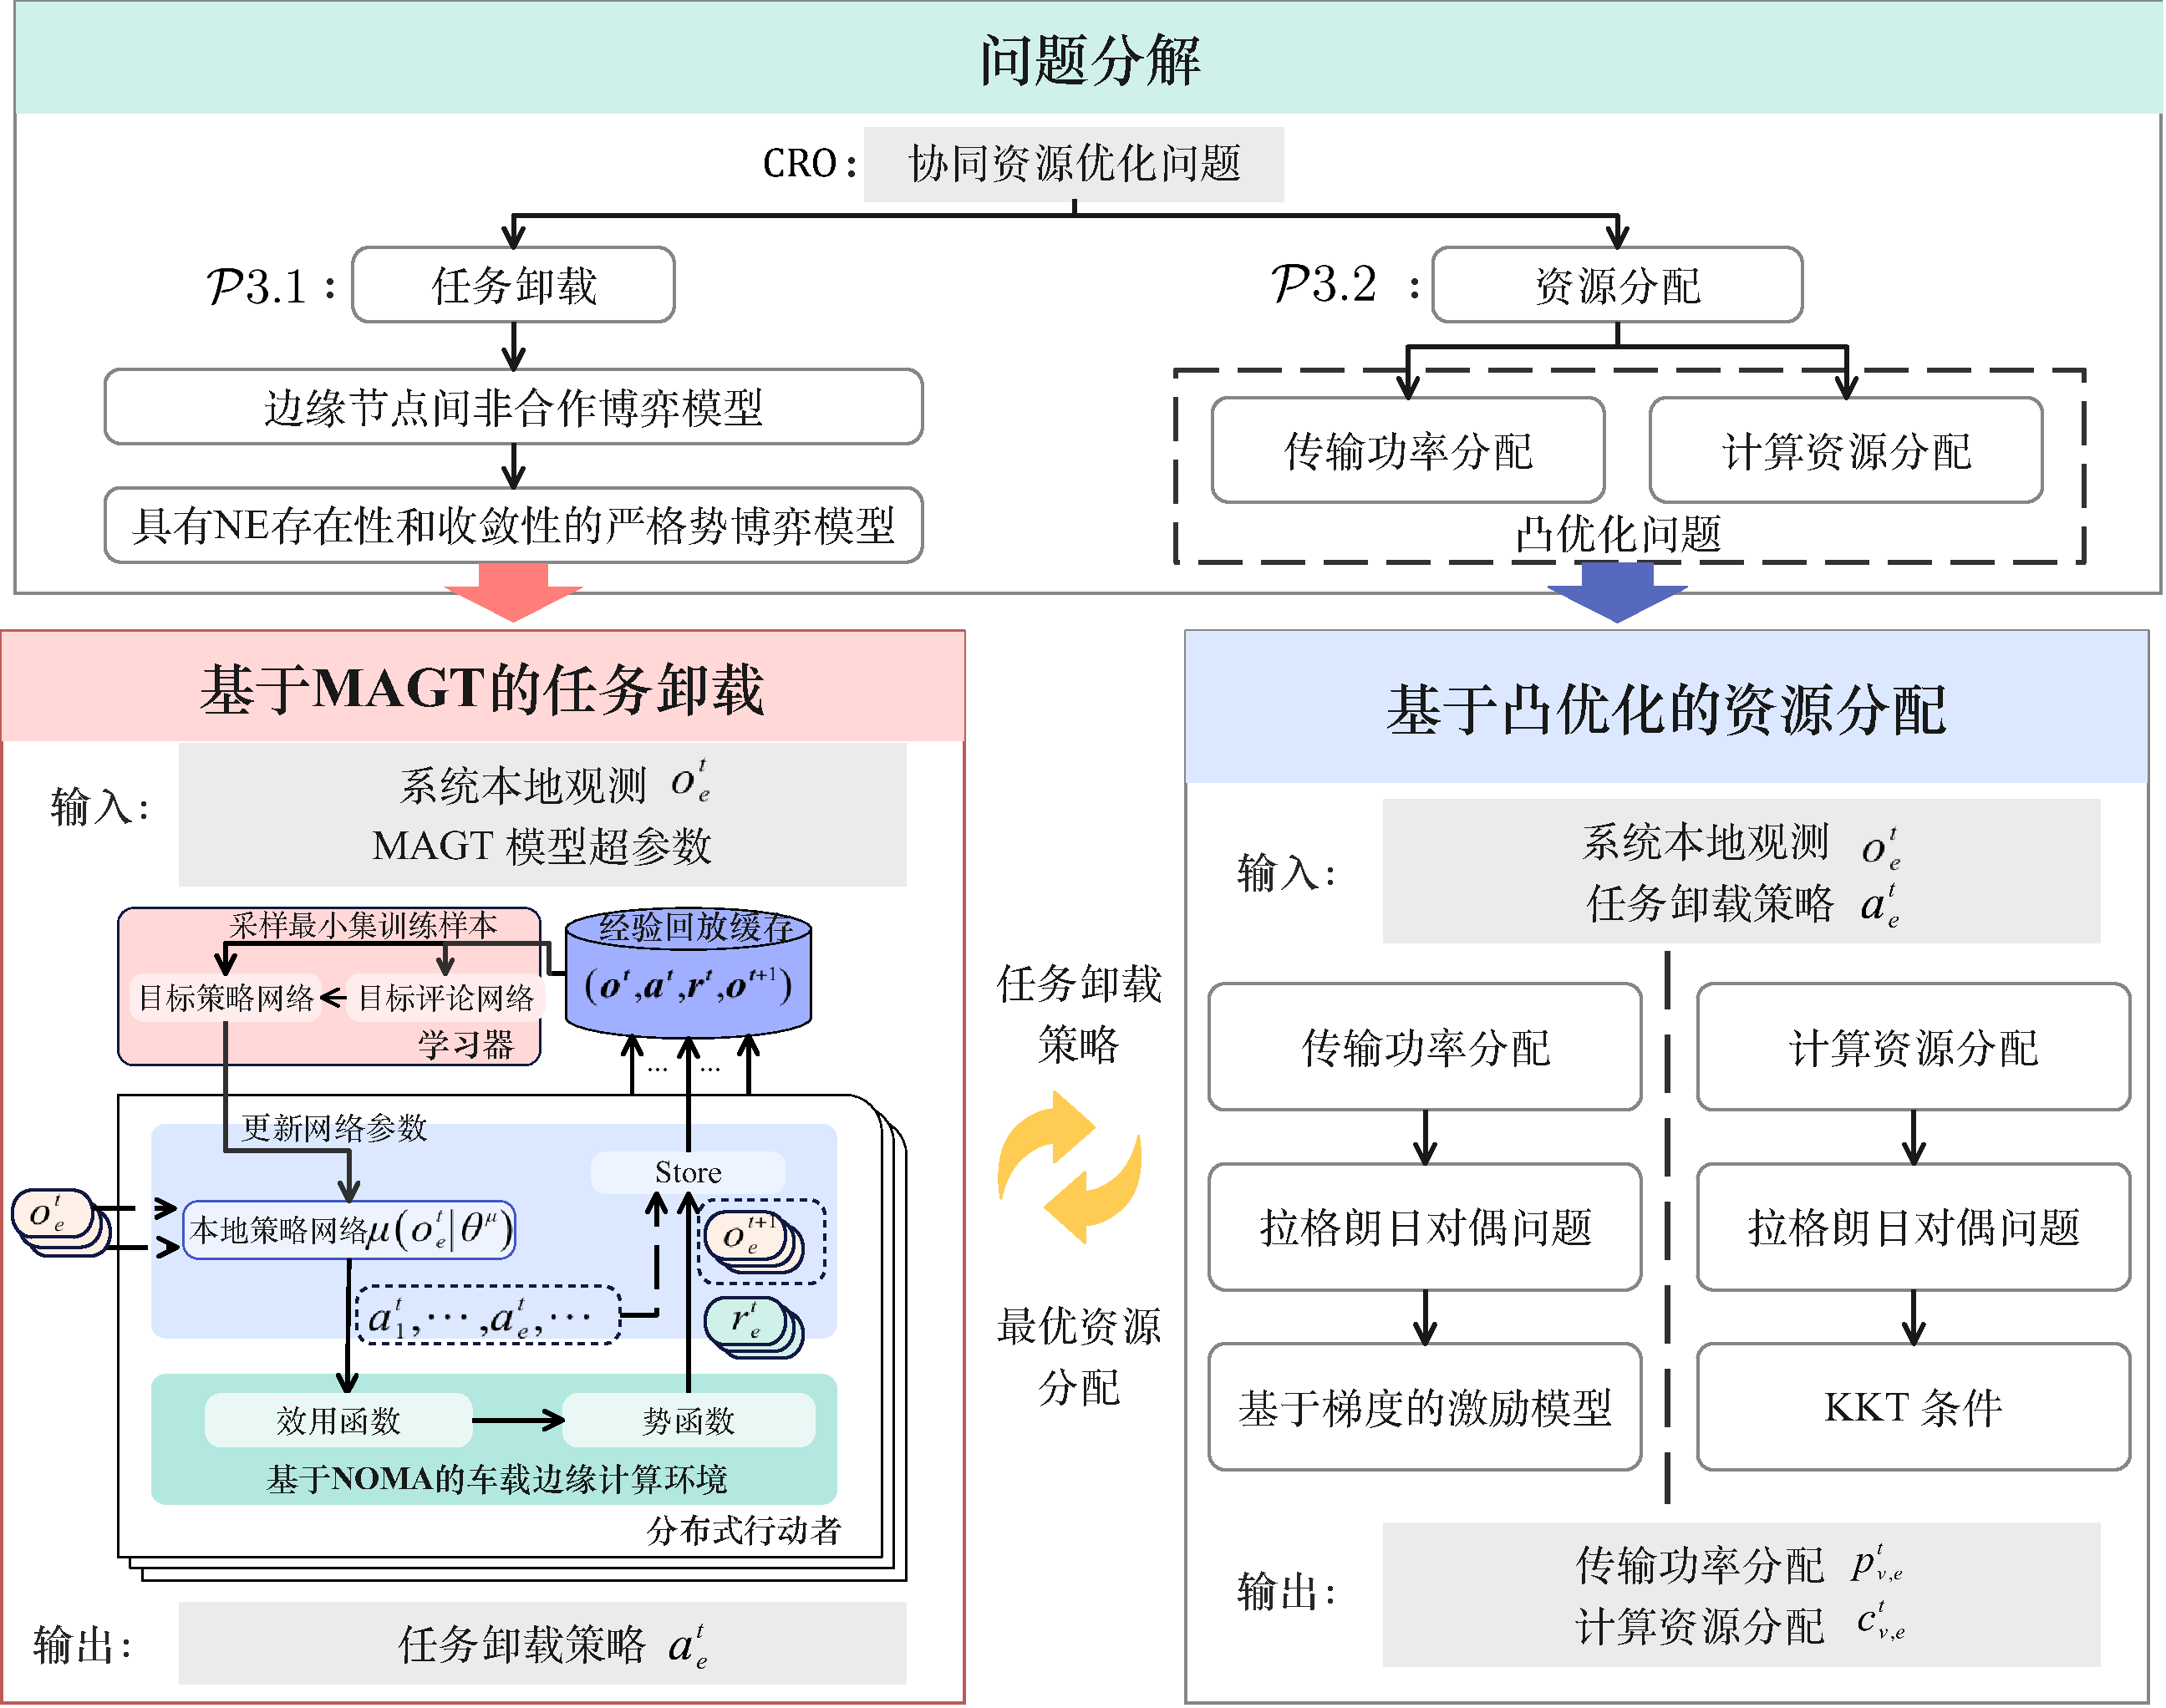
\includegraphics[width=1\columnwidth]{Fig3-3-solution-model.pdf}
  \bicaption{基于博弈理论的多智能体深度深度强化学习算法模型}{Multi-agent game-theoretic deep reinforcement learning model}
  \label{fig 3-3}
\end{figure} 

\subsection{问题分解}
在本节中,首先将CRO分解为单个时间片的多个问题。
由于$\mathbf{P}^{t}$、$\mathbf{Q}^{t}$和$\mathbf{C}^{t}$在时间$t$的变量是相互独立的,并且变量不重叠,四个约束条件是可分离的,所以CRO可以分解为两个子问题,其表述如下:

\textbf{1) 任务卸载:} 第一个任务卸载子问题$\mathcal{P}3.1$只涉及边缘节点的任务卸载决策$\mathbf{Q}^{t}$,其表述为
\begin{equation}
	\begin{aligned}
		\mathcal{P}3.1: &\max_{\mathbf{Q}^{t}} g_1= \sum_{ \forall e \in \mathbf{E}} \Psi_{e}^{t}  \\
		\text { s.t. }  
		&\mathcal{C}3.5: q_{v, e}^t \in \left \{0, 1\right \}, \forall v \in \mathbf{V}, \forall e \in \mathbf{E}  \\
        &\mathcal{C}3.6: \sum_{\forall e \in \mathbf{E}} q_{v, e}^t = 1, \forall v \in \mathbf{V} \\
	\end{aligned}
\end{equation}
然后,将 $\mathcal{P}3.1$ 建模为边缘节点之间的非合作博弈,其中边缘节点作为玩家,独立决定任务卸载策略。
该博弈模型表示为
\begin{equation}
	\mathcal{G} = \left\{\mathbf{E}, \mathbb{S}, \left\{{U}_{e}\right\}_{\forall e \in \mathbf{E}} \right\}
\end{equation}
其中$\mathbf{E}$表示玩家的集合;
$\mathbb{S}$ 表示博弈的策略空间,其被定义为所有边缘节点的单独策略集的笛卡尔乘积,即$\mathbb{S} = \mathbf{S}_{1} \times \ldots \times \mathbf{S}_{e} \times \ldots \times \mathbf{S}_{E}$,其中$\mathbf{S}_{e}$表示边缘节点$e$的所有可能策略集。
$\mathbb{S}$中的每个元素$\mathcal{S}$都是一个具体策略,$\mathcal{S} = \left(\mathcal{S}_{1}, \ldots, \mathcal{S}_{e}, \ldots, \mathcal{S}_{E} \right)$,并可以改写为 $\mathcal{S}=\left( \mathcal{S}_{e}, \mathcal{S}_{-e}\right)$,其中 $\mathcal{S}_{-e}$ 表示边缘节点 $e$ 的对手(即$\forall e^{\prime} \in \mathbf{E} \setminus \{e\}$)所采取的联合策略。
而$\mathcal{S}_{e}$是边缘节点$e$的策略,可以用$\mathcal{S}_{e} = \left\{ q_{v, e}^t \mid \forall e \in \mathbf{E}, \forall v \in \mathbf{V}_{e}^{t} \right\}$表示。
${U}_{e}\left(\mathcal{S}\right)$表示边缘节点$e$的效用函数,其定义如下:
\begin{definition}
边缘节点$e$的效用函数用${U}_{e}\left(\mathcal{S}\right): \mathbb{S} \mapsto \mathbb{R}$表示, 其被定义为策略概况下$\mathcal{S}$边缘节点的服务率之和,其中$\mathbb{R}$为实数集。
	\begin{equation}
		{U}_{e}\left(\mathcal{S}\right) = \sum_{\forall e \in \mathbf{E}} \Psi_{e}^{t}
	\end{equation}
\end{definition}

此外,本章通过给定一个势函数如公式\ref{equ 3-16}所示,证明该非合作博弈模型$\mathcal{G}$是一个具有NE存在和收敛性的EPG。
\begin{theorem}
给定边缘节点 $e$的势函数如下
\begin{equation}
	{F}_{e}\left(\mathcal{S}\right) = {U}_{e}\left(\mathcal{S}_{e}, \mathcal{S}_{-e}\right) - {U}_{e}\left(-\mathcal{S}_{e}, \mathcal{S}_{-e}\right)
	\label{equ 3-16}
\end{equation}
该博弈 $\mathcal{G}$ 是一个严格势博弈。
\label{theorem 4-1}
\end{theorem}
\noindent 其中${U}_{e}\left(-\mathcal{S}_{e}, \mathcal{S}_{-e}\right)$是边缘节点$e$的策略无效时的效用值。
\begin{proof} 见附录 \ref{appendix f}。
\end{proof}
\noindent 在博弈模型$\mathcal{G}$中,边缘节点试图在利益冲突的情况下通过最大化其效用来实现纳什均衡 \cite{chew2016potential}。
\begin{definition}
策略$\mathcal{S}^{*} \in \mathbb{S}$是一个纯策略的纳什均衡\cite{chew2016potential}当且仅当
	\begin{equation}
		U_{e}\left(\mathcal{S}_{e}^{*}, \mathcal{S}_{-e}^{*}\right) \geq U_{e}\left(\mathcal{S}_{e}, \mathcal{S}_{-e}^{*}\right), \quad \forall \mathcal{S}_{e} \in \mathbf{S}_{e}, \forall e \in \mathbf{E}
	\end{equation}
\end{definition}
\begin{lemma}
	给定一个势函数 $F_{e}(\mathcal{S})$ 如公式\ref{equ 3-16}所示,博弈 $\mathcal{G}$ 的NE 集合恰好和博弈$\mathcal{G}^{F}=\left\{\mathbf{E}, \mathbb{S}, \left\{{F}_{e}\right\}_{\forall e \in \mathbf{E}} \right\}$的NE集合一致,即
	\begin{equation}
		\mathcal{NE}(\mathcal{G}) \equiv \mathcal{NE}\left(\mathcal{G}^{F}\right)
	\end{equation}
	其中 $\mathcal{NE}$ 表示博弈模型的NE集合。
\label{lemma 4-1}
\end{lemma}
\begin{proof} 见附录 \ref{appendix g}。
\end{proof}
\noindent 最后, 本章基于引理\ref{lemma 4-1}证明博弈模型 $\mathcal{G}$ 具有纳什均衡的存在性。
\begin{theorem}
	给定势函数 $F_{e}(\mathcal{S})$ 如公式 \ref{equ 3-16},博弈 $\mathcal{G}$ 至少有一个纯策略的NE。
\label{theorem 4-2}
\end{theorem}
\begin{proof} 见附录 \ref{appendix h}。
\end{proof}
\noindent 另一方面,由于策略空间$\mathbb{S}$有限,NE可以在有限的步骤中收敛。
本章建立了$\epsilon$改进路径和$\epsilon$平衡点\cite{chew2016potential},其为一个近似于真实NE的策略,然后证明NE的收敛性。
\begin{definition} 
	路径 $\rho=\left(\mathcal{S}^{0}, \mathcal{S}^{1}, \mathcal{S}^{2}, \ldots\right)$ 是 $\epsilon$改进路径 \cite{chew2016potential},当其向前进任何一步 $i$,边缘节点 $e$ 的效能都提升了$\epsilon$,即 $U_{e}\left(\mathcal{S}^{i+1}\right) > U_{e}\left(\mathcal{S}^{i}\right) + \epsilon, \exists \epsilon \in \mathbb{R}_{+}, \forall i$。
\end{definition}
\begin{definition}
	策略 $\mathcal{\hat{S}} \in \mathbb{S}$ 是一个 $\epsilon$均衡 \cite{chew2016potential} 当且仅当 $\exists \epsilon \in \mathbb{R}_{+}$,并且
	\begin{equation}
		U_{e}\left(\mathcal{\hat{S}}_{e}, \mathcal{\hat{S}}_{-e}\right) \geq U_{e}\left(\mathcal{S}_{e}, \mathcal{\hat{S}}_{-e}\right) - \epsilon, \quad \forall \mathcal{S}_{e} \in \mathbf{S}_{e}, \forall e \in \mathbf{E}
	\end{equation}
\end{definition}
\begin{theorem}
对于博弈$\mathcal{G}$,每条$\epsilon$改进路径的步数都是有限的,其终点是$\epsilon$均衡,其是对原始NE的改进。
\label{theorem 4-3}
\end{theorem}
\begin{proof} 见附录 \ref{appendix i}。
\end{proof}

\textbf{2) 资源分配:} 第二个子问题$\mathcal{P}3.2$涉及传输功率分配$\mathbf{P}^{t}$和计算资源分配$\mathbf{C}^{t}$,其表述如下
\begin{align}
	\mathcal{P}3.2: &\min_{\mathbf{P}^{t}, \mathbf{C}^{t}} g_2= \sum_{ \forall e \in \mathbf{E}} \sum_{\forall k_{v}^{t} \in \mathbf{K}_{e}^{t}} \left( m_{v, e}^{t} +  n_{v, e}^{t} \right) \notag \\
	\text { s.t. }
    &\mathcal{C}3.7: \sum_{\forall v \in \mathbf{V}_{e}^{t}} p_{v, e}^{t} \leq p_{e}, \forall e \in \mathbf{E} \notag \\
    &\mathcal{C}3.8: \sum_{\forall k_{v}^{t} \in {\mathbf{K}_{q_e}^{t} }} c_{v, e}^t \leq c_{e}, \forall e \in \mathbf{E}
\label{equ 3-21}
\end{align}

\noindent 可以看出,公式\ref{equ 3-21}中的$\mathbf{P}^{t}$和$\mathbf{C}^{t}$的变量是相互独立的。
同时,因为变量没有重叠,限制条件$\mathcal{C}3.7$和$\mathcal{C}3.8$是可分离的。
因此,子问题$\mathcal{P}3.2$可以分为两个独立的问题,即传输功率分配和计算资源分配,其表述如下:

\textbf{传输功率分配:} 其只涉传输功率分配变量$\mathbf{P}^{t}$,其表述如下
\begin{align}
	\mathcal{P}3.3: &\min_{\mathbf{P}^{t}} g_3= \sum_{ \forall e \in \mathbf{E}} \sum_{\forall k_{v}^{t} \in \mathbf{K}_{e}^{t}}  \frac{d_{k}}{b  \log _{2}\left(1+\mathrm{SINR}_{v, e}^t\right)} \notag \\
	&\text { s.t. } \mathcal{C}3.7: \sum_{\forall v \in \mathbf{V}_{e}^{t}} p_{v, e}^{t} \leq p_{e}, \forall e \in \mathbf{E}
\end{align}
显然,与边缘节点相关的变量是独立的。
因此,$\mathcal{P}3.3$可以进一步划分为多个简单问题,其中每个问题只与单个边缘节点$e$有关。
\begin{align}
	\mathcal{P}3.4: & \max_{\mathbf{P}_{e}^{t}}  g_3^e= \sum_{\forall k_{v}^{t} \in \mathbf{K}_{e}^{t}} {b  \log _{2}\left(1+\mathrm{SINR}_{v, e}^t\right)} \notag \\
	&\text { s.t. } \mathcal{C}3.9: \sum_{\forall v \in \mathbf{V}_{e}^{t}} p_{v, e}^{t} \leq p_{e}  
\end{align}
然而,由于边缘内和边缘间的干扰,$\mathcal{P}3.4$是非凸的。
然后,本章应用近似方法将$\mathcal{P}3.4$转换成一个凸问题。
特别地,$g_3^e$的下界可以通过下式得到\cite{papandriopoulos2006low}。
\begin{equation}
	g_3^e \geq \overline{g_3^e} = \sum_{\forall k_{v}^{t} \in \mathbf{K}_{e}^{t}} {b \left( \xi_{v, e}^{t} \log _{2}\mathrm{SINR}_{v, e}^t + \omega_{v, e}^{t} \right) }
\end{equation}
其中,$\xi_{v, e}^{t}$ 和 $\omega_{v, e}^{t}$ 是固定值并由下式给出。
\begin{align}
	\xi_{v, e}^{t} &= \overline{\mathrm{SINR}}_{v, e}^t \bigg/ ( 1 + \overline{\mathrm{SINR}}_{v, e}^t ) \\
	\omega_{v, e}^{t} &= \log _{2} (1+ \overline{\mathrm{SINR}}_{v, e}^t) - \frac{\overline{\mathrm{SINR}}_{v, e}^t}{1 + \overline{\mathrm{SINR}}_{v, e}^t} \log _{2}\overline{\mathrm{SINR}}_{v, e}^t
\end{align}
如果${\mathrm{SINR}}_{v, e}^t =\overline{\mathrm{SINR}}_{v, e}^t$,该下界是紧的。
因此,$\mathcal{P}3.4$可以松弛后重新表达为
\begin{align}
	\mathcal{P}3.5: & \max_{\mathbf{P}_{e}^{t}}  \overline{g_3^e}= \sum_{\forall k_{v}^{t} \in \mathbf{K}_{e}^{t}} {b \left( \xi_{v, e}^{t} \log _{2}\mathrm{SINR}_{v, e}^t + \omega_{v, e}^{t} \right) } \notag \\
	&\text { s.t. } \mathcal{C}3.9: \sum_{\forall v \in \mathbf{V}_{e}^{t}} p_{v, e}^{t} \leq p_{e}  
\end{align}
尽管如此,$\mathcal{P}3.5$仍然是非凸的,因为目标在$\mathbf{P}_{e}^{t}$中不是凹的。
给定一个新的变量$\widetilde{p_{v, e}^t} = \log _{2} {p}_{v, e}^t$,$\mathcal{P}3.5$可以被转化为如下形式
\begin{align}
	\mathcal{P}3.6: & \max_{\widetilde{\mathbf{{P}}_{e}^{t}}}  \widetilde{g_3^{e}}= \sum_{\forall k_{v}^{t} \in \mathbf{K}_{e}^{t}} {b ( \xi_{v, e}^{t} \log _{2}\mathrm{\widetilde{SINR}}_{v, e}^t + \omega_{v, e}^{t} ) } \notag \\
	&\text { s.t. } \mathcal{C}3.10: \sum_{\forall v \in \mathbf{V}_{e}^{t}} 2^{\widetilde{p_{v, e}^t}} \leq p_{e}  
\end{align}
其中 $\log _{2}\mathrm{\widetilde{SINR}}_{v, e}^t$ 由以下公式给出
\begin{align}
	\log _{2}\mathrm{\widetilde{SINR}}_{v, e}^t &= \widetilde{p_{v, e}^t} + \log _{2} |h_{v, e}^t| ^{2} - \log _{2} \left( \sum\limits_{\forall v^{\prime} \in \mathbf{V}_{h_{v, e}}^{t}} |h_{v^{\prime}, e}^t|^2 2^{\widetilde{p_{v^{\prime}, e}^{t}}} \right. \notag \\
	&+ \left. \sum\limits_{\forall e^{\prime} \in \mathbf{E} / \{e\}} \sum\limits_{\forall v^{\prime} \in \mathbf{V}_{e^{\prime}}^{t}} |h_{v^{\prime}, e}^t|^2 2^{\widetilde{p_{v^{\prime}, e^{\prime}}^{t}}} + N_{0}\right)
\end{align}
\noindent 因此,$\mathcal{P}3.6$是一个标准的凹最大化问题,也是一个凸优化问题,因为每个约束条件都是凸型指数之和,而目标之和中的每项都是凹的。

\textbf{计算资源分配:} 其是关于$\mathbf{C}^{t}$变量的计算资源分配,其表述如下
\begin{align}
	\mathcal{P}3.7: &\min_{\mathbf{C}^{t}} g_4= \sum_{ \forall e \in \mathbf{E}} \sum_{\forall k_{v}^{t} \in \mathbf{K}_{e}^{t}} ( w_{v, e}^{t} + \sum_{\forall e^{\prime} \in \mathbf{E}} q_{v, e^{\prime}}^{t} x_{v, e^{\prime}}^t) \notag \\
	&\text { s.t. } \mathcal{C}3.8:  \sum_{\forall k_{v}^{t} \in {\mathbf{K}_{q_e}^{t} }} c_{v, e}^t \leq c_{e}, \forall e \in \mathbf{E}
\end{align}
与公式中的$\mathcal{P}3.3$类似,$\mathcal{P}3.7$可以进一步分解为多个简单问题,每个问题只与一个边缘节点$e$有关,其表述如下
\begin{align}
	\mathcal{P}3.8: &\min_{\mathbf{C}_{e}^{t}} g_4^e= \sum_{\forall a_{v}^{t} \in {\mathbf{K}_{q_e}^{t} }}   x_{v, e}^t \notag \\
	&\text { s.t. } \mathcal{C}3.11:  \sum_{\forall k_{v}^{t} \in {\mathbf{K}_{q_e}^{t} }} {c_{v, e}^t} \leq c_{e}
\label{equ 3-29}
\end{align}
\noindent 其中${\mathbf{C}_e^t}$代表${\mathbf{C}^{t}}$中与边缘节点$e$相关的变量。
因此,$\mathcal{P}3.8$是一个凸优化问题,因为公式\ref{equ 3-29} 中的目标是凸的,而约束是线性的。

\subsection{基于MAGT的任务卸载}
MAGT模型由若干个分布式行动者、一个学习器、一个基于NOMA的VEC环境和一个经验回放缓存组成。
MAGT的主要组成部分设计如下:

\textbf{1) 系统状态:} 边缘节点$e$在时间$t$上对系统状态的局部观察被表示为
	\begin{equation}
		\boldsymbol{o}_{e}^{t}=\left\{e, t, \mathbf{Dis}_{\mathbf{V}_{e}^{t}}, \mathbf{D}_{\mathbf{K}_{e}^{t}}, \mathbf{C}_{\mathbf{K}_{e}^{t}}, \mathbf{T}_{\mathbf{K}_{v}^{t}}\right\}
	\end{equation} 
	\noindent 其中$e$是边缘节点索引;
	$t$是时隙索引;
	$\mathbf{Dis}_{\mathbf{V}_{e}^{t}}$代表$e$在时间$t$的边缘节点和车辆$v \in \mathbf{V}_{e}^{t}$之间的距离集合;
	$\mathbf{D}_{\mathbf{K}_{e}^{t}}$、$\mathbf{C}_{\mathbf{K}_{e}^{t}}$和$\mathbf{T}_{\mathbf{K}_{v}^{t}}$分别代表$t$时边缘节点$e$中的$k_{v}^{t} \in \mathbf{K}_{e}^{t}$的数据大小、所需计算资源和截止时间。
	因此,时间$t$的系统状态可表示为$\boldsymbol{o}^{t}=\left\{\boldsymbol{o}_{1}^{t}, \ldots, \boldsymbol{o}_{e}^{t}, \ldots, \boldsymbol{o}_{E}^{t}\right\}$。

\textbf{2) 动作空间:} 边缘节点$e$的动作空间由车辆$v \in \mathbf{V}_{e}^{t}$请求任务的卸载决策组成,其表示为
	\begin{equation}
		\boldsymbol{a}_{e}^{t} = \left\{ q_{v, e^{\prime}}^t \mid \forall e^{\prime} \in \mathbf{E}, \forall v \in \mathbf{V}_{e}^{t} \right\}
	\end{equation}
	\noindent 其中,$q_{v, e^{\prime}}^t \in \{0, 1\}$表示任务$k_{v}^t$是否在边缘节点$e^{\prime}$中被卸载。
	边缘节点动作的集合表示为 $\boldsymbol{a}^{t} = \left\{\boldsymbol{a}_{e}^{t}\mid \forall e \in \mathbf{E} \right\}$.
	
\textbf{3) 奖励函数:} 在博弈模型中,每个边缘节点的目标是使其效用最大化。
	因此,系统的奖励函数被定义为边缘节点在时间$t$实现的效用,其表示方法为
	\begin{equation}
		r\left(\boldsymbol{a}^{t} \mid \boldsymbol{o}^{t}\right)= {U}_{e}\left(\mathcal{S}_{e}, \mathcal{S}_{-e}\right) = \sum_{\forall e \in \mathbf{E}} \Psi_{e}^{t}
		\label{equ 3-32}
	\end{equation}
	此外,博弈$\mathcal{G}$ 的势函数被采纳为边缘节点在系统状态$\boldsymbol{o}^{t}$下的行动$\boldsymbol{a}_{e}^{t}$的奖励。
	\begin{equation}
		r_{e}^{t} = r\left(\boldsymbol{a}^{t} \mid \boldsymbol{o}^{t}\right)-r\left(\boldsymbol{a}_{-e}^{t} \mid \boldsymbol{o}^{t}\right)
		\label{equ 3-33}
	\end{equation}
	\noindent 其中$r\left(\boldsymbol{a}_{-e}^{t} \mid \boldsymbol{o}^{t}\right)$是在没有边缘节点$e$贡献的情况下实现的系统奖励,它可以通过设置边缘节点$e$的空动作集得到。
	边缘节点的奖励集合用$\boldsymbol{r}^{t} = \{r_{1}^{t}, \ldots, r_{e}^{t}, \ldots, r_{E}^{t}\}$。
	在MAGT中,每个边缘节点 $e \in \mathbf{E}$的目标是最大化预期收益,用$R_{e}^{t} = \sum_{i \geq 0} \gamma^{i} r_{e}^{t+i}$表示,其中$\gamma$是折扣系数。

在MAGT的开始阶段,本地策略和评论家网络的参数在学习器中被随机初始化,其分别用 $\theta^{\mu}$和$\theta^{Q}$表示。
然后,目标策略和评论家网络的参数被初始化为与相应的本地网络相同,分别用$\theta^{\mu^{\prime}}$和$\theta^{Q^{\prime}}$表示。
\begin{align}
	\theta^{\mu^{\prime}} \leftarrow \theta^{\mu}\\
	\theta^{Q^{\prime}} \leftarrow \theta^{Q}
\end{align}
而经验回放缓存$\mathcal{B}$被初始化为最大存储大小$|\mathcal{B}|$,以存储回放经验。

\SetKwInOut{KwIn}{输入}
\SetKwInOut{KwOut}{输出}

\begin{algorithm}[h]\small
\renewcommand{\algorithmcfname}{算法}
	\caption{基于博弈理论的多智能深度强化学习}
\KwIn{折扣因子 $\gamma$、批大小 $M$、样本长度 $N$、回放经验缓存 $\mathcal{B}$、探索常数 $\epsilon$、学习率$\alpha$和$\beta$、目标网络参数更新周期 $t_{\operatorname{tgt}}$、分布式行动者网络参数更新周期 $t_{\operatorname{act}}$}
\KwOut{任务卸载决策$q_{v, e^{\prime}}^t$、传输功率分配策略$p_{v, e}^{t, {(i+1)}}$、计算资源分配策略${c_{v, e}^{t}}^{\star}$}
	初始化网络参数\\
	初始化经验回放缓存 $\mathcal{B}$\\
	\For{\songti{分布式行动体} $j = 1$ \songti{到} $J$}{
			初始化一个随机过程 $\mathcal{N}$ 以进行探索\\
			行动体从学习器中复制网络参数\\
			接收初始系统状态 $\boldsymbol{o}_{1}$\\
			\For{\songti{时间片} $t = 1$ \songti{到} $T$}{
				\For{\songti{边缘节点} $e=1$ \songti{到} $E$}{
					接收本地观测 $\boldsymbol{o}_{e}^{t}$\\
					选择一个动作 $\boldsymbol{a}_{e}^{t}=\boldsymbol{\mu}\left(\boldsymbol{o}_{e}^{t} \mid \theta^{\mu}_{j}\right)+\mathcal{N}_{t}$\\
					基于梯度的迭代方法得到最优传输功率分配\\
					基于KKT条件得到最优计算资源分配\\
				}
				接收奖励 $\boldsymbol{r}^{t}$ 和下一个系统状态 $\boldsymbol{o}^{t+1}$\\
				存储 $\left(\boldsymbol{o}^{t}, \boldsymbol{a}^{t}, \boldsymbol{r}^{t}, \boldsymbol{o}^{t+1}\right)$ 到经验回放缓存 $\mathcal{B}$;
			}
	}
	\For{\songti{迭代次数} $= 1$ \songti{到最大迭代次数}}{
		\For{\songti{时间片} $t = 1$ \songti{到} $T$}{
			\For{\songti{边缘节点} $e=1$ \songti{到} $E$}{
				从经验回放缓存$\mathcal{B}$随机采样长度为$N$ 的$M$ 最小样本集\\
				构建目标分布\\
				计算策略和评论家网络损失\\
				更新本地策略和评论家网络
			}
			\If{$t \mod t_{\operatorname{tgt}} = 0$}{
				更新目标网络\\
			}
			\If{$t \mod t_{\operatorname{act}} = 0$}{
				复制网络参数给分布式行动者
			}
		}
	}
\label{algorithm 3-1}
\end{algorithm}

另一方面,$J$个分布式行动者通过与环境同时交互而产生重放经验。
第$j$个角色的本地策略网络的参数是从学习器的本地策略网络中复制得到的,用$\theta^{\mu}_{j}$表示。
每次迭代的初始化系统状态用$\boldsymbol{o}^{0}$表示。
根据对系统状态的局部观察,得到第$j$个行为体中的边缘节点$e$在时间$t$的任务卸载动作。
\begin{equation}
	\boldsymbol{a}_{e}^{t}={\mu}\left(\boldsymbol{o}_{e}^{t} \mid \theta^{\mu}_{j}\right)+\epsilon  \mathcal{N}_{t}
\end{equation}
\noindent 其中,$\mathcal{N}_{t}$为探索噪声,以增加边缘行动的多样性,$\epsilon$为探索常数。
然后,边缘节点的动作$\boldsymbol{a}^{t}$在基于NOMA的VEC环境中执行,每个边缘节点的奖励可以根据公式\ref{equ 3-33}得到。
最后,包括当前系统状态$\boldsymbol{o}^{t}$、边缘节点动作$\boldsymbol{a}^{t}$、边缘节点奖励$\boldsymbol{r}^{t}$和下一时刻系统状态$\boldsymbol{o}^{t+1}$在内的交互经验被存储到经验回放缓存$\mathcal{B}$。
迭代将继续进行,直到学习器完成训练过程。

从经验回放缓存$\mathcal{B}$中抽取长度为$N$的$M$样本的小批量,以训练学习器的策略和评论家网络。
$M$小批量中样本用$\left(\boldsymbol{o}^{i:i+N}, \boldsymbol{a}^{i:i+N-1}, \boldsymbol{r}^{i:i+N-1}\right)$来表示。
边缘节点$e$的目标分布用$Y_e^i$表示,其计算方法为:
\begin{equation}
	Y_e^{i} = \sum_{n=0}^{N-1} \left( \gamma^{n} r_{e}^{i+n}\right)+\gamma^{N} Q^{\prime}\left(\boldsymbol{o}_{e}^{i+N}, \boldsymbol{a}^{i+N} \mid \theta^{Q^{\prime}} \right)
\end{equation}
\noindent 其中 $\boldsymbol{a}^{i+N} = \{ \boldsymbol{a}_{1}^{i+N}, \ldots, \boldsymbol{a}_{e}^{i+N}, \ldots, \boldsymbol{a}_{E}^{i+N} \}$ 且 $\boldsymbol{a}_{e}^{i+N}$ 是通过目标策略网络得到的, 即$\boldsymbol{a}_{e}^{i+N} = \mu^{\prime}(\boldsymbol{o}_{e}^{i+N} \mid \theta^{\mu^{\prime}})$。
评论家网络的损失函数表示为
\begin{equation}
	{L}\left(\theta^{Q}\right)=\frac{1}{M} \sum_{i} \frac{1}{E} \sum_{e} \left(Y_e^{i}-Q\left(\boldsymbol{o}_{e}^{i}, \boldsymbol{a}^{i} \mid \theta^{Q}\right)\right)^{2}
\end{equation}
策略网络的参数通过策略梯度进行更新。
\begin{equation}
	\nabla_{\theta^{\mu}} \mathcal{J} = \frac{1}{M} \sum_{i} \frac{1}{E} \sum_{e} \nabla_{\boldsymbol{a}_{e}^{i}} Q\left(\boldsymbol{o}_{e}^{i}, \boldsymbol{a}^{i} \mid \theta^{Q}\right) \nabla_{\theta^{\mu}} \mu\left(\boldsymbol{o}_{e}^{i} \mid \theta^{\mu}\right)
\end{equation}
本地策略网络和本地评论家网络的参数以学习率$\alpha$和$\beta$更新。
最后,如果$t\mod t_{\operatorname{tgt}}=0$,边缘节点更新目标网络的参数,其中$t_{\operatorname{tgt}}$为目标网络参数更新周期。
\begin{align}
	\theta^{\mu^{\prime}} &\leftarrow n \theta^{\mu}+(1-n)  \theta^{\mu^{\prime}}\\
	\theta^{Q^{\prime}} &\leftarrow n  \theta^{Q}+(1-n) \theta^{Q^{\prime}}
\end{align}
\noindent 其中 $n \ll 1$。
第$j$个行为者的策略网络参数也会定期更新,即当$t \mod t_{\operatorname{act}} = 0$时,其中$t_{\operatorname{act}}$是分布式行为者的网络参数更新周期。
\begin{equation}
	\theta_{j}^{\mu} \leftarrow \theta^{\mu^{\prime}}, \forall j
\end{equation}
其中$\theta_{j}^{\mu}$表示第$j$个分布式行为体中的本地策略网络参数。
	
\subsection{基于凸优化的资源分配}
\textbf{1) 传输功率分配:} 为了解决凸优化问题$\mathcal{P}3.6$,本章首先利用拉格朗日对偶法\cite{boyd2004convex},在$\mathcal{P}3.6$中引入拉格朗日乘数$\lambda_{e}^{t}$,拉格朗日函数如下:
\begin{equation}
	\mathcal{L}(\widetilde{\mathbf{{P}}_{e}^{t}}, {\lambda}_{e}^{t} ) = \widetilde{g_3^{e}} -  {\lambda}_{e}^{t} (\sum_{\forall v \in \mathbf{V}_{e}^{t}} 2^{\widetilde{p_{v, e}^{t}}} - p_{e} )
	\label{equ 3-41}
\end{equation}
此外,$\mathcal{P}3.6$的对偶问题可表示为:
\begin{align}
	\mathcal{P}3.9: & \min_{{\lambda}_{e}^{t}} \max_{\widetilde{\mathbf{{P}}_{e}^{t}}}  g_5 = \mathcal{L}(\widetilde{\mathbf{{P}}_{e}^{t}}, {\lambda}_{e}^{t} ) \notag \\
	&\text { s.t. } \mathcal{C}3.12: \mathbf{\lambda}_{e}^{t} \geq 0  
\end{align}
因此,$\mathcal{P}3.9$可以分解为两层优化问题。
内层表示为固定${\lambda}_{e}^{t}$的$\widetilde{\mathbf{{P}}_{e}^{t}}$的优化问题,外层表示为固定$\widetilde{\mathbf{{P}}_{e}^{t}}$的${\lambda}_{e}^{t}$优化问题。
在外层,对偶变量${\lambda}_{e}^{t}$通过梯度下降迭代更新。
\begin{equation}
	\mathbf{\lambda}_{e}^{t, (i+1)} = \max\left\{0, \mathbf{\lambda}_{e}^{t, (i)} + \sigma (\sum_{\forall v \in \mathbf{V}_{e}^{t}} 2^{\widetilde{p_{v, e}^{t}}} - p_{e} )\right\}
\end{equation}
其中$\widetilde{p_{v, e}^{t}}$是固定的;$\sigma$是一个足够小的常数,$i$是一个迭代次数。
此外,内部对偶最大化可以通过寻找公式\ref{equ 3-41}中拉格朗日函数静止点来解决,即相对于$\widetilde{\mathbf{{P}}_{e}^{t}}$固定${\lambda}_{e}^{t}$。
\begin{equation}
\frac{\partial \mathcal{L}\left(\widetilde{\mathbf{{P}}_{e}^{t}}, \mathbf{\lambda}_{e}^{t} \right)}{\partial \widetilde{p_{v, e}^{t}}}= b  \xi_{v, e}^{t}  - p_{v, e}^{t}(\lambda_{e}^{t} +\sum\limits_{\forall v^{\prime} \in \mathbf{V}_{h_{v, e}}^{t}} b  \xi_{v, e}^{t} |h_{v, e}^t|^2 \frac{\mathrm{SINR}_{v^{\prime}, e}^t}{|h_{v^{\prime}, e}^t| ^{2} p_{v^{\prime}, e}^{t}}) =0
\end{equation}
其中,偏导数被转换回$\mathbf{P}_{e}^{t}$空间。
因此,可以列出定点方程,车辆$v$的传输功率通过以下方式更新。
\begin{equation}
p_{v, e}^{t, {(i+1)}}=\frac{b \xi_{v, e}^{t}}{\lambda_{e}^{t,(i)}+\sum\limits_{\forall v^{\prime} \in \mathbf{V}_{h_{v, e}}^{t}} b  \xi_{v, e}^{t}|h_{v, e}^t|^2 {I}_{v^{\prime}, e}^{t, (i)} }
\end{equation}
其中$\lambda_{e}^{t,(i)}$和$p_{v, e}^{t, (i+1)}$分别表示$\lambda_{e}^{t}$和$p_{v, e}^{t}$在$i$次迭代的值,${I}_{v^{\prime}, e}^{t, (i)}$由如下公式给出。
\begin{equation}
	{I}_{v^{\prime}, e}^{t, (i)} = \sum\limits_{\forall v^{\prime} \in \mathbf{V}_{h_{v, e}}^{t}} |h_{v^{\prime}, e}^t|^2 p_{v^{\prime}, e}^{t, (i)} + \sum\limits_{\forall e^{\prime} \in \mathbf{E} / \{e\}} \sum\limits_{\forall v^{\prime} \in \mathbf{V}_{e^{\prime}}^{t}} |h_{v^{\prime}, e}^t|^2 p_{v^{\prime}, e^{\prime}}^{t, (i)} + N_{0}
\end{equation}
其中 $p_{v^{\prime}, e}^{t, (i)}$ 和 $p_{v^{\prime}, e^{\prime}}^{t, (i)}$ 分别表示 $p_{v^{\prime}, e}^{t}$ 和 $p_{v^{\prime}, e^{\prime}}^{t}$ 在 $i$次迭代的值。

\textbf{2) 计算资源分配:} 与传输功率分配类似,本章首先在$\mathcal{P}3.8$中引入拉格朗日乘数${\lambda}_{e}^{t}$。
然后,$\mathcal{P}3.8$的对偶问题可以表示为
\begin{align}
	\mathcal{P}3.10: & \min_{\mathbf{\lambda}_{e}^{t}, \mathbf{{C}}_{e}^{t}}  g_6 = g_4^e - {\lambda}_{e}^{t} (\sum_{\forall k_{v}^{t} \in {\mathbf{K}_{q_e}^{t} }} {c_{v, e}^t} - c_{e} ) \notag \\
		&\text { s.t. } \mathcal{C}3.12: \mathbf{\lambda}_{e}^{t} \geq 0 
\end{align}
基于KKT条件\cite{boyd2004convex},可以得到以下公式。
\begin{align}
	\nabla_{\mathbf{C}_e^{t}} g_4^e + \mathbf{\lambda}_{e}^{t}\nabla_{\mathbf{C}_e^{t}} (\sum_{\forall k_{v}^{t} \in {\mathbf{K}_{q_e}^{t} }} {c_{v, e}^t} - c_{e} ) &= 0, \notag \\
	\mathbf{\lambda}_{e}^{t}( \sum_{\forall k_{v}^{t} \in {\mathbf{K}_{q_e}^{t} }} {c_{v, e}^t} - {c_{e}} ) &= 0, \notag \\
	\mathbf{\lambda}_{e}^{t} &\geq 0
\end{align}
通过求解方程组,可以得到任务$k_{v}^{t}$的计算资源分配的最优方案如下:
\begin{equation}
	{c_{v, e}^{t}}^{\star} = \frac{1 / c_e \sqrt{d_k  c_k} } {\sum_{\forall k_{v}^{t} \in {\mathbf{K}_{q_e}^{t} }} 1 / c_e \sqrt{d_k  c_k}} , \forall k_{v}^{t} \in {\mathbf{K}_{q_e}^{t} } 
\end{equation}

\section{实验结果与分析}\label{section 3-5}

\subsection{实验设置}

在本章节中,本章通过使用Python 3.9.13和TensorFlow 2.8.0实现了一个仿真模型,以评估所提出的解决方案的性能。
仿真模型基于Ubuntu 20.04服务器,其配备AMD Ryzen 9 5950X 16核处理器(时钟频率为3.4 GHz),两个NVIDIA GeForce RTX 3090图形处理单元,以及64 GB内存。
本章考虑在一个3平方千米的正方形区边缘内的一般情况,其中$E=9$边缘节点,如5G基站和RSU均匀分布在场景图上。
在参考 \inlinecite{zhu2021decentralized}、 \inlinecite{liu2021rtds}、 \inlinecite{xu2021socially}和\inlinecite{zhou2019computation}的基础上,仿真实验参数设置如下:
边缘节点的计算能力(即CPU时钟频率)被设定为均匀分布在$[3, 10]$ GHz \cite{zhou2019computation}。 
V2I通信的通信范围被设定为$u_e =$ 500 m\cite{zhu2021decentralized}。
此外,利用现实的车辆轨迹作为交通输入,从滴滴GAIA开放数据集中提取2016年11月16日中国成都市青羊区3平方千米区域的数据。
特别地,本章研究了四个不同时期(即8:00-8:05、13:00-13:05、18:00-18:05,以及23:00-23:05)的服务场景。

为了实现MAGT,策略和评论家网络结构描述如下:
本地策略网络是一个有三个隐藏层的五层全连接神经网络,其中神经元的数量分别为256、256和256。
目标策略网络的结构与本地策略网络相同。
本地评论家网络是一个五层全连接神经网络,有三个隐藏层,其中神经元的数量分别是512、512和256。
目标批评家网络的结构与本地批评家网络相同。
利用ReLU作为激活函数,并使用Adam优化器来更新网络权重。
分布式行动者的数量设定为$J$=10。
主要的系统模型参数和算法参数显示在表\ref{table 3-1}和\ref{table 3-2}中。

\begin{table}[h]\small
\centering
\bicaption{系统模型参数}{Parameters of system model}
\setlength{\tabcolsep}{15mm}{
\begin{tabular}[t]{ccc}
\toprule
参数&值\\
\midrule
请求任务大小 $d_k$ \cite{liu2021rtds}&[0.01, 5] MB\\
处理1 bit 任务数据所需的计算资源 $c_k$ \cite{zhu2021decentralized} & 500 cycles/bit\\
任务的截止时间 $t_k$  \cite{liu2021rtds}&[5, 10] s\\
V2I 带宽 $b$ \cite{zhou2019computation}&20 MHz\\
边缘节点的计算能力 $c_e$ \cite{zhou2019computation}&[3, 10] GHz\\
V2I 通信最大传输功率 $p_e$ \cite{zhu2021decentralized}&1$\times 10^3$ mW\\
V2I 通信范围 $u_e$ \cite{zhu2021decentralized}&500 m\\
有线传输速率 $z$&50 Mbps\\
距离折扣 $\zeta$& 6.667$\times 10^{-4}$\\
加性白高斯噪声 $N_0$ \cite{xu2021socially}&-90 dBm\\
大尺度路径损耗指数 $\varphi$ \cite{xu2021socially}&3\\
\bottomrule
\end{tabular}}
\label{table 3-1}
\end{table}

\begin{table}[h]\small
\centering
\bicaption{MAGT模型参数}{Parameters of MAGT}
\setlength{\tabcolsep}{18.5mm}{
\begin{tabular}[t]{ccc}
\toprule
参数&值\\
\midrule
折扣因子 $\gamma$&0.996\\
批大小 $M$&256\\
回放缓存最大容量 $|\mathcal{B}|$&1$\times10^{6}$\\
探索常数 $\epsilon$&0.3\\
策略网络和评价家网络的学习率&1$\times10^{-4}$\\
目标网络参数更新周期 $t_{\operatorname{tgt}}$&100\\
分布式行动者网络参数更新周期 $t_{\operatorname{act}}$&1000\\
\bottomrule
\end{tabular}}
\label{table 3-2}
\end{table}
 
为了进行性能比较,本章实现了以下四种可比的算法。
\begin{itemize}
	\item \textbf{最优资源分配和任务全迁移}: 其分为两个阶段:资源分配和任务卸载。其中资源分配问题通过凸优化得到最优解,同时边缘节点倾向于将所有任务迁移到其他边缘节点。
	\item \textbf{最优资源分配和任务仅本地处理}: 其中资源分配与ORM算法相同,同时每个边缘节点倾向于在本地执行所有任务。
	\item \textbf{分布式深度确定性策略梯度} \cite{barth2018distributed}: 其通过实现一个以全局系统状态为输入的DDPG智能体,共同决定任务卸载决策、V2I传输功率分配和计算资源分配,其中效用函数被作为智能体的奖励。
	\item \textbf{多智能体深度确定性策略梯度}\cite{zhang2021adaptive}: 其中资源分配与ORM算法相同,并在每个边缘节点中实现MADDPG,以独立确定任务卸载决策,其中效用函数被作为边缘节点的奖励。
\end{itemize}

为了进行性能评估,本章收集以下统计数据。每个任务的上传时间和处理时间;本地执行的任务总数,用$K_{\operatorname{local}}$表示;迁移到其他边缘节点的任务数,用$K_{\operatorname{migrated}}$表示;任务总数,用$K_{\operatorname{total}}$表示,以及服务的任务数,用$K_{\operatorname{serviced}}$表示。
在此基础上,根据公式\ref{equ 3-9}、\ref{equ 3-10}、\ref{equ 3-11}和 \ref{equ 3-32}得到四个指标,即\textbf{平均处理时间}、\textbf{平均服务时间}、\textbf{平均服务率}(Average Service Ratio, ASR)和\textbf{累积奖励}。
本章进一步设计了以下两个额外的度量来进行分析。
\begin{itemize}
	\item \textbf{平均实现势} : 它被定义为边缘奖励的总和(即实现的势)除以调度期间的边缘节点数,其计算公式为:
		\begin{equation}
		 	 \operatorname{AAP} = \frac{1}{E}\sum_{\forall e \in \mathbf{E}} \sum_{\forall t \in \mathbf{T}} r_{e}^{t}
		\end{equation}
	\item \textbf{本地处理与迁移的比例} : 本地处理的任务的比例可通过下式计算:
		\begin{equation}
			P_{\operatorname{local}} = \frac{K_{\operatorname{local}}}{K_{\operatorname{total}}}
		\end{equation}
		而迁移到其他边缘节点的任务的比例计算如下:
		\begin{equation}
			P_{\operatorname{migrated}} = \frac{K_{\operatorname{migrated}}}{K_{\operatorname{total}}}
		\end{equation}
		且 $P_{\operatorname{local}} +P_{\operatorname{migrated}} = 1$。
\end{itemize}

\subsection{实验结果与分析}

\textbf{1) 算法收敛性:} 图\ref{fig 3-4}比较了五种算法在不同交通场景下的收敛性能以及CR。如图所示,MAGT的收敛速度仅次于D4PG(即3000次左右的迭代),但它却取得了最高的CR值(即230左右)。相比之下,D4PG和MADDPG分别经过2000和3500次左右的迭代后收敛,并实现了190和220左右的CR。而ORL和ORM分别实现了约210和189的CR。据观察,ORM、ORL、MADDPG和MAGT在前2000次迭代中可以达到比D4PG高得多的CR。主要原因是在ORM、ORL、MADDPG和MAGT中使用了提出的最优资源分配方案,使其性能优于共同决定任务卸载和资源分配的D4PG。另一方面,由于在MAGT中利用分布式行为者加速重放经验采样,所提出的解决方案比MADDPG收敛得更快,同时在不同的交通场景下实现了最高CR。

\begin{figure}[h]
\centering
  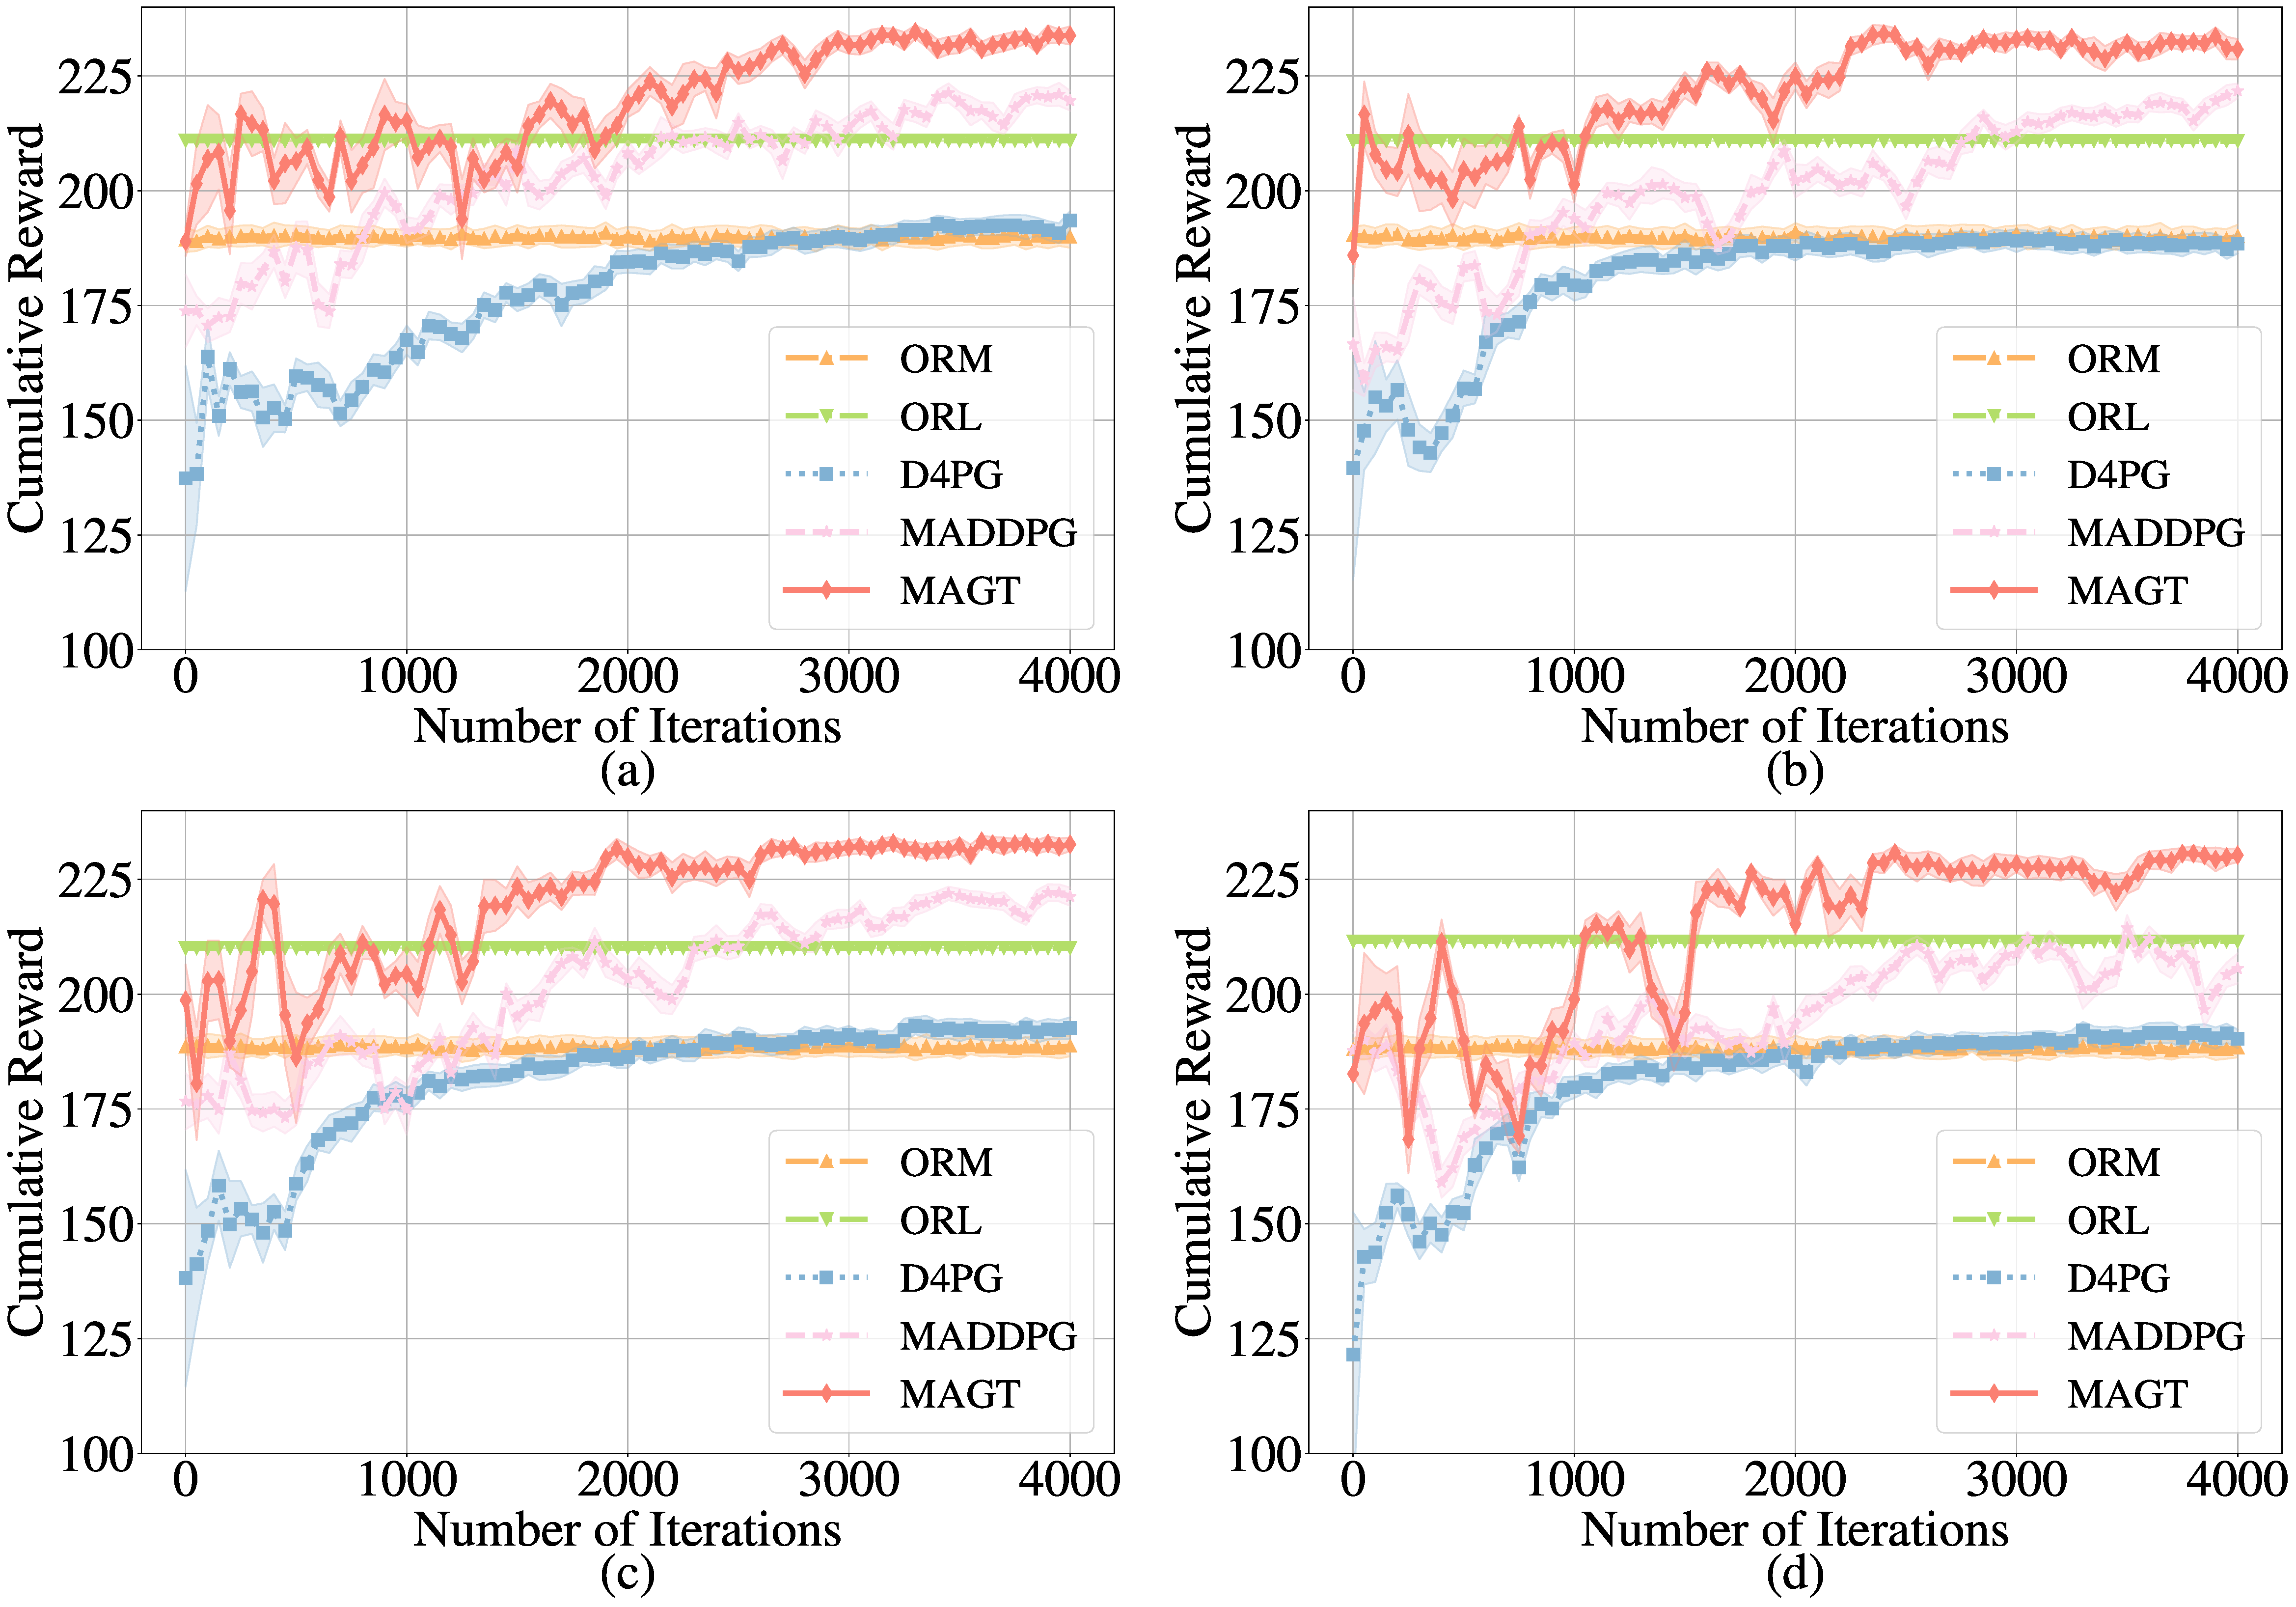
\includegraphics[width=1\columnwidth]{Fig3-4-convergence.pdf}
  \bicaption[不同交通场景下的算法收敛性]{不同交通场景下的算法收敛性。(a)场景1(b)场景2(c)场景3(d)场景4}[Algorithm convergence under different traffic scenarios]{Algorithm convergence under different traffic scenarios. (a) Scenario 1 (b) Scenario 2 (c) Scenario 3 (d) Scenario 4}
  \label{fig 3-4}
\end{figure} 

\textbf{2) 交通场景的影响:} 图\ref{fig 3-5}比较了不同交通场景下的五种算法。如图所示,图\ref{fig 3-5}(a)比较了五种算法的ASR,MAGT实现了最高的ASR。图\ref{fig 3-5}(b) 比较了五种算法的CR。如上所述,MAGT的CR高于ORM、ORL、D4PG和MADDPG。图\ref{fig 3-5}(c) 比较了五种算法的AAP。MAGT在所有场景下都能达到最高的AAP,这表明MAGT中采用势函数作为边缘节点奖励的优势。图\ref{fig 3-5}(d) and \ref{fig 3-5}(e)分别比较了五种算法的AST和APT。其表明,MAGT可以实现边缘节点之间的合作通信和计算,通过最小化任务的平均服务时间来提高整体服务率。正如预期,MAGT的APT是最低的。这可以从图\ref{fig 3-5}(f) 中得到进一步验证,图中显示任务更有可能迁移到其他边缘节点以获得更快的处理。

\begin{figure}[h]
\centering
  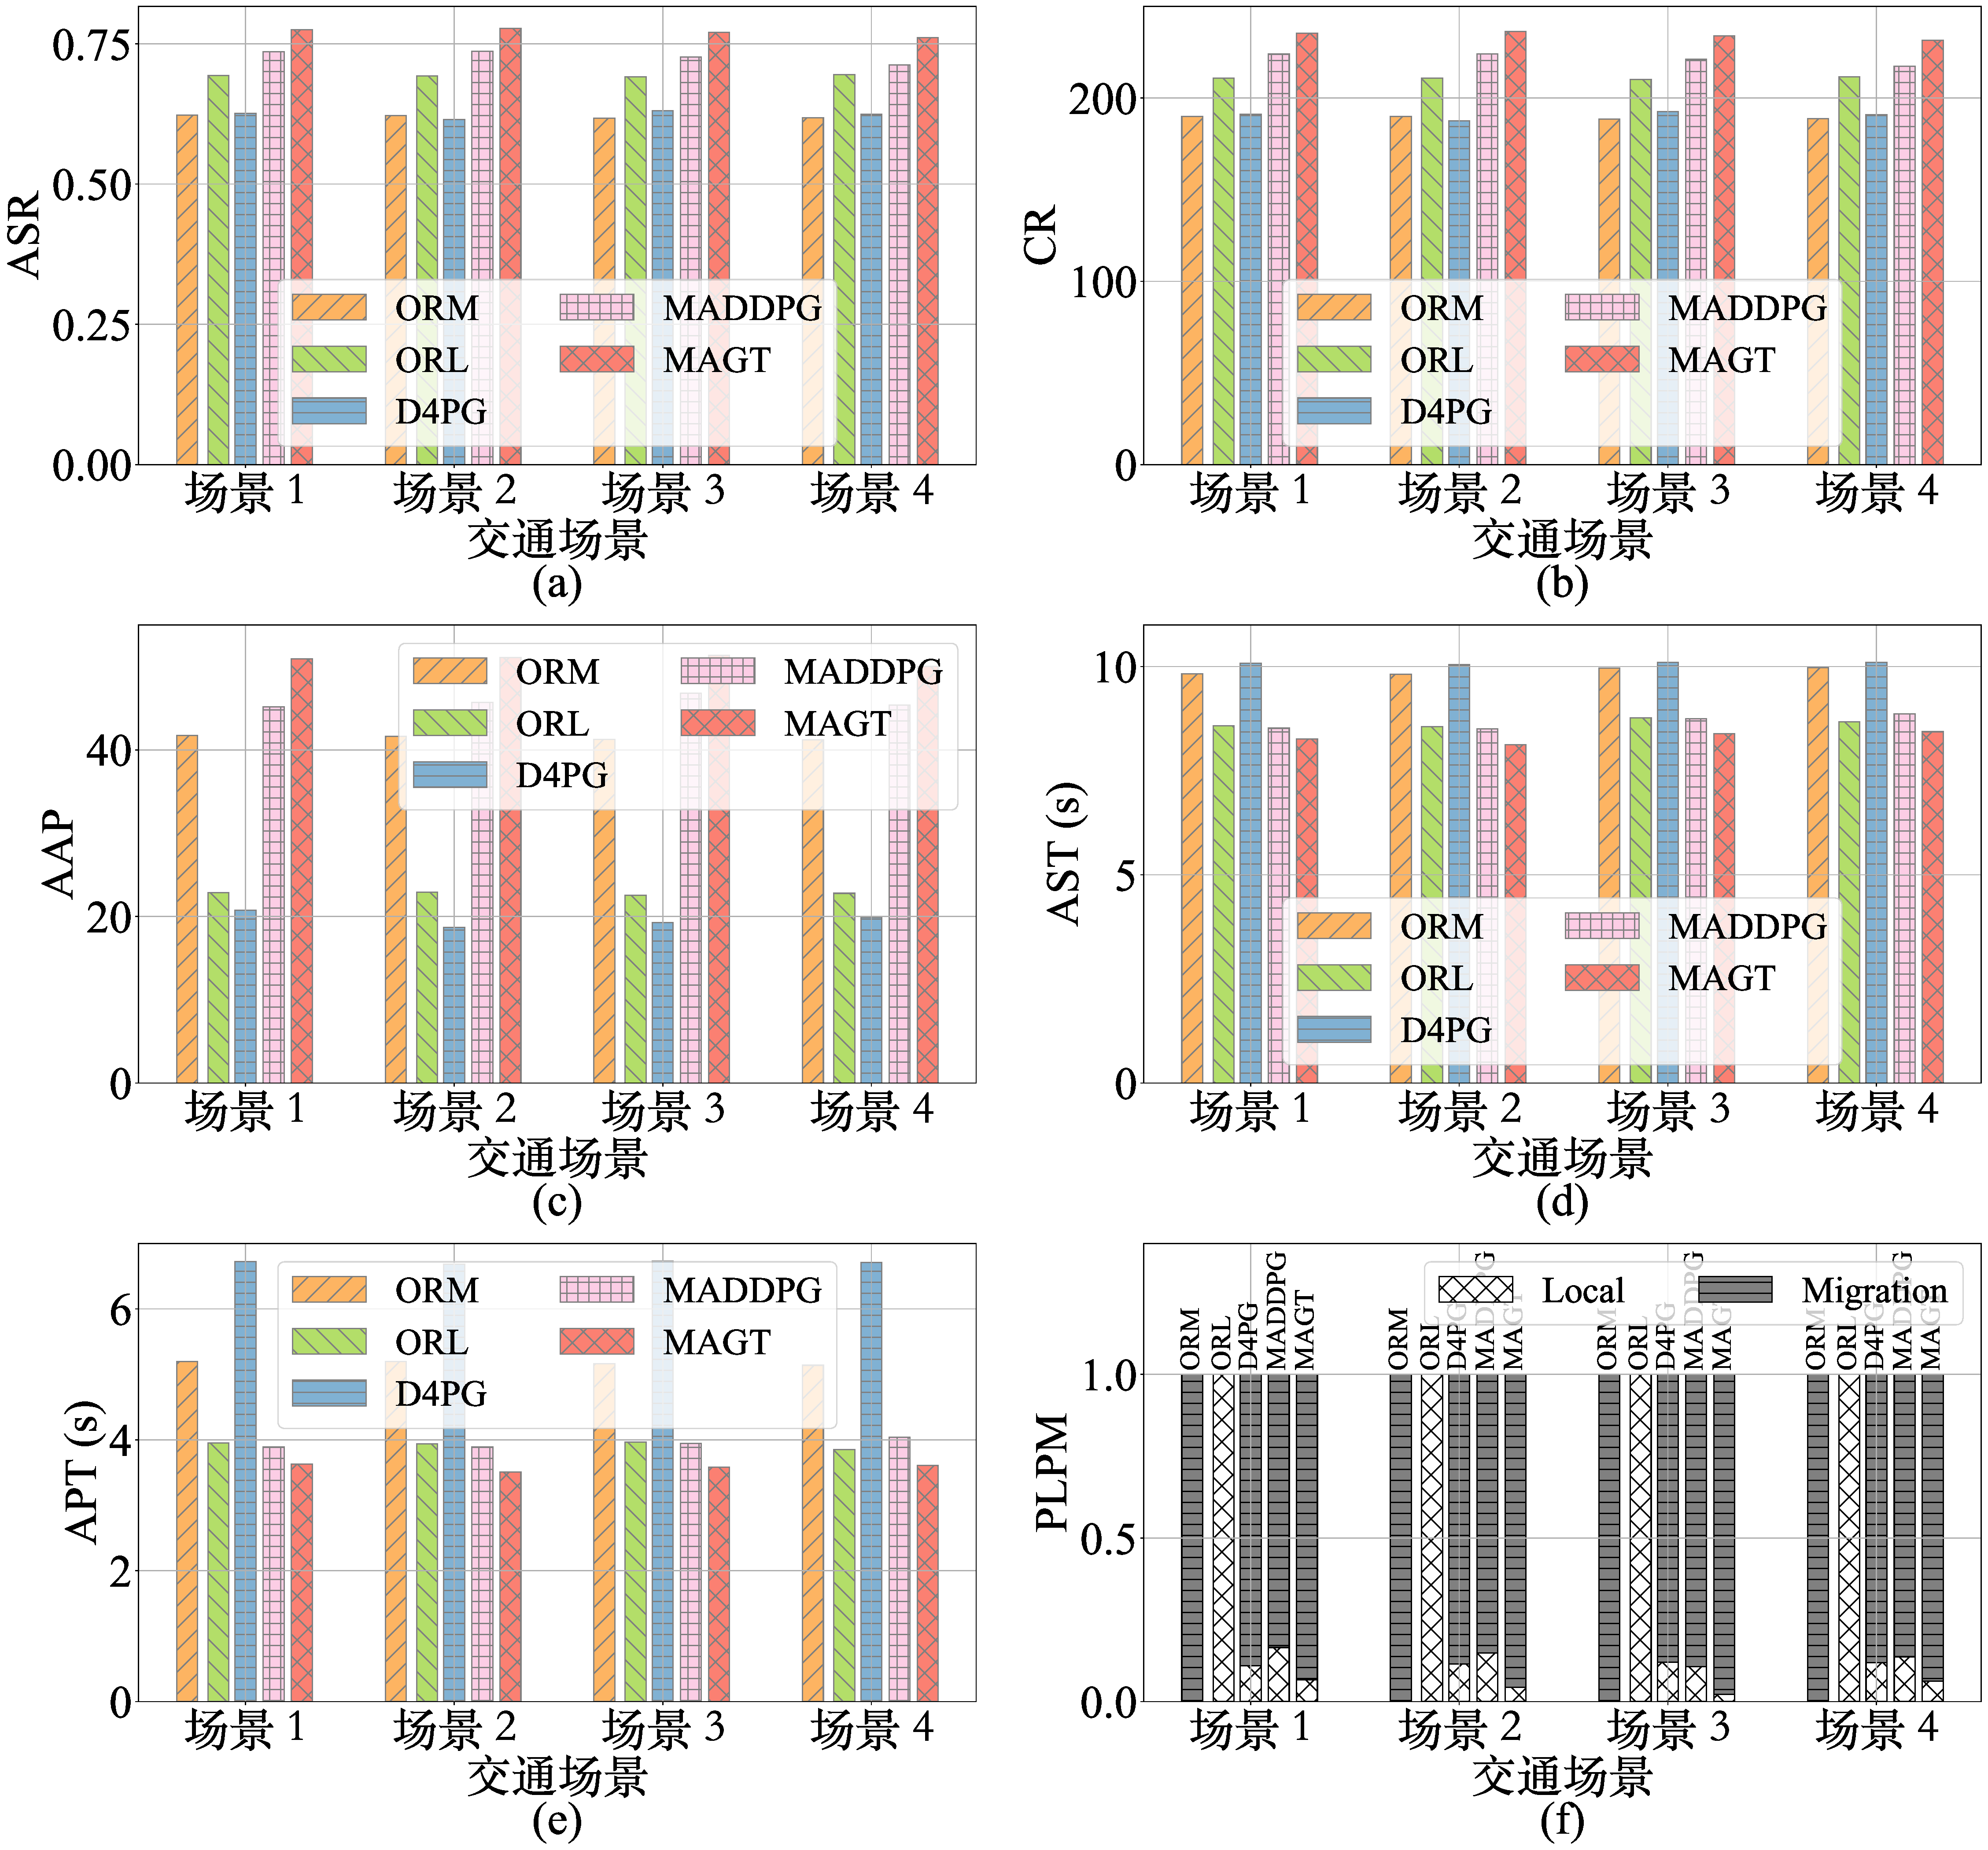
\includegraphics[width=1\columnwidth]{Fig3-5-different-traffica-scenarios.pdf}
  \bicaption[不同交通场景下的性能比较]{不同交通场景下的性能比较。(a)平均服务率(b)累积奖励(c)平均实现势(d)平均服务时间(e)平均处理时间(f)本地处理与迁移的比例}[Performance comparison under different traffic scenarios]{Performance comparison under different traffic scenarios. (a) Average service ratio (b) Cumulative reward (c) Average achieved potential (d) Average service time (e) Average processing time (f) Proportion of local processing to migration}
  \label{fig 3-5}
\end{figure}

\begin{figure}[h]
\centering
  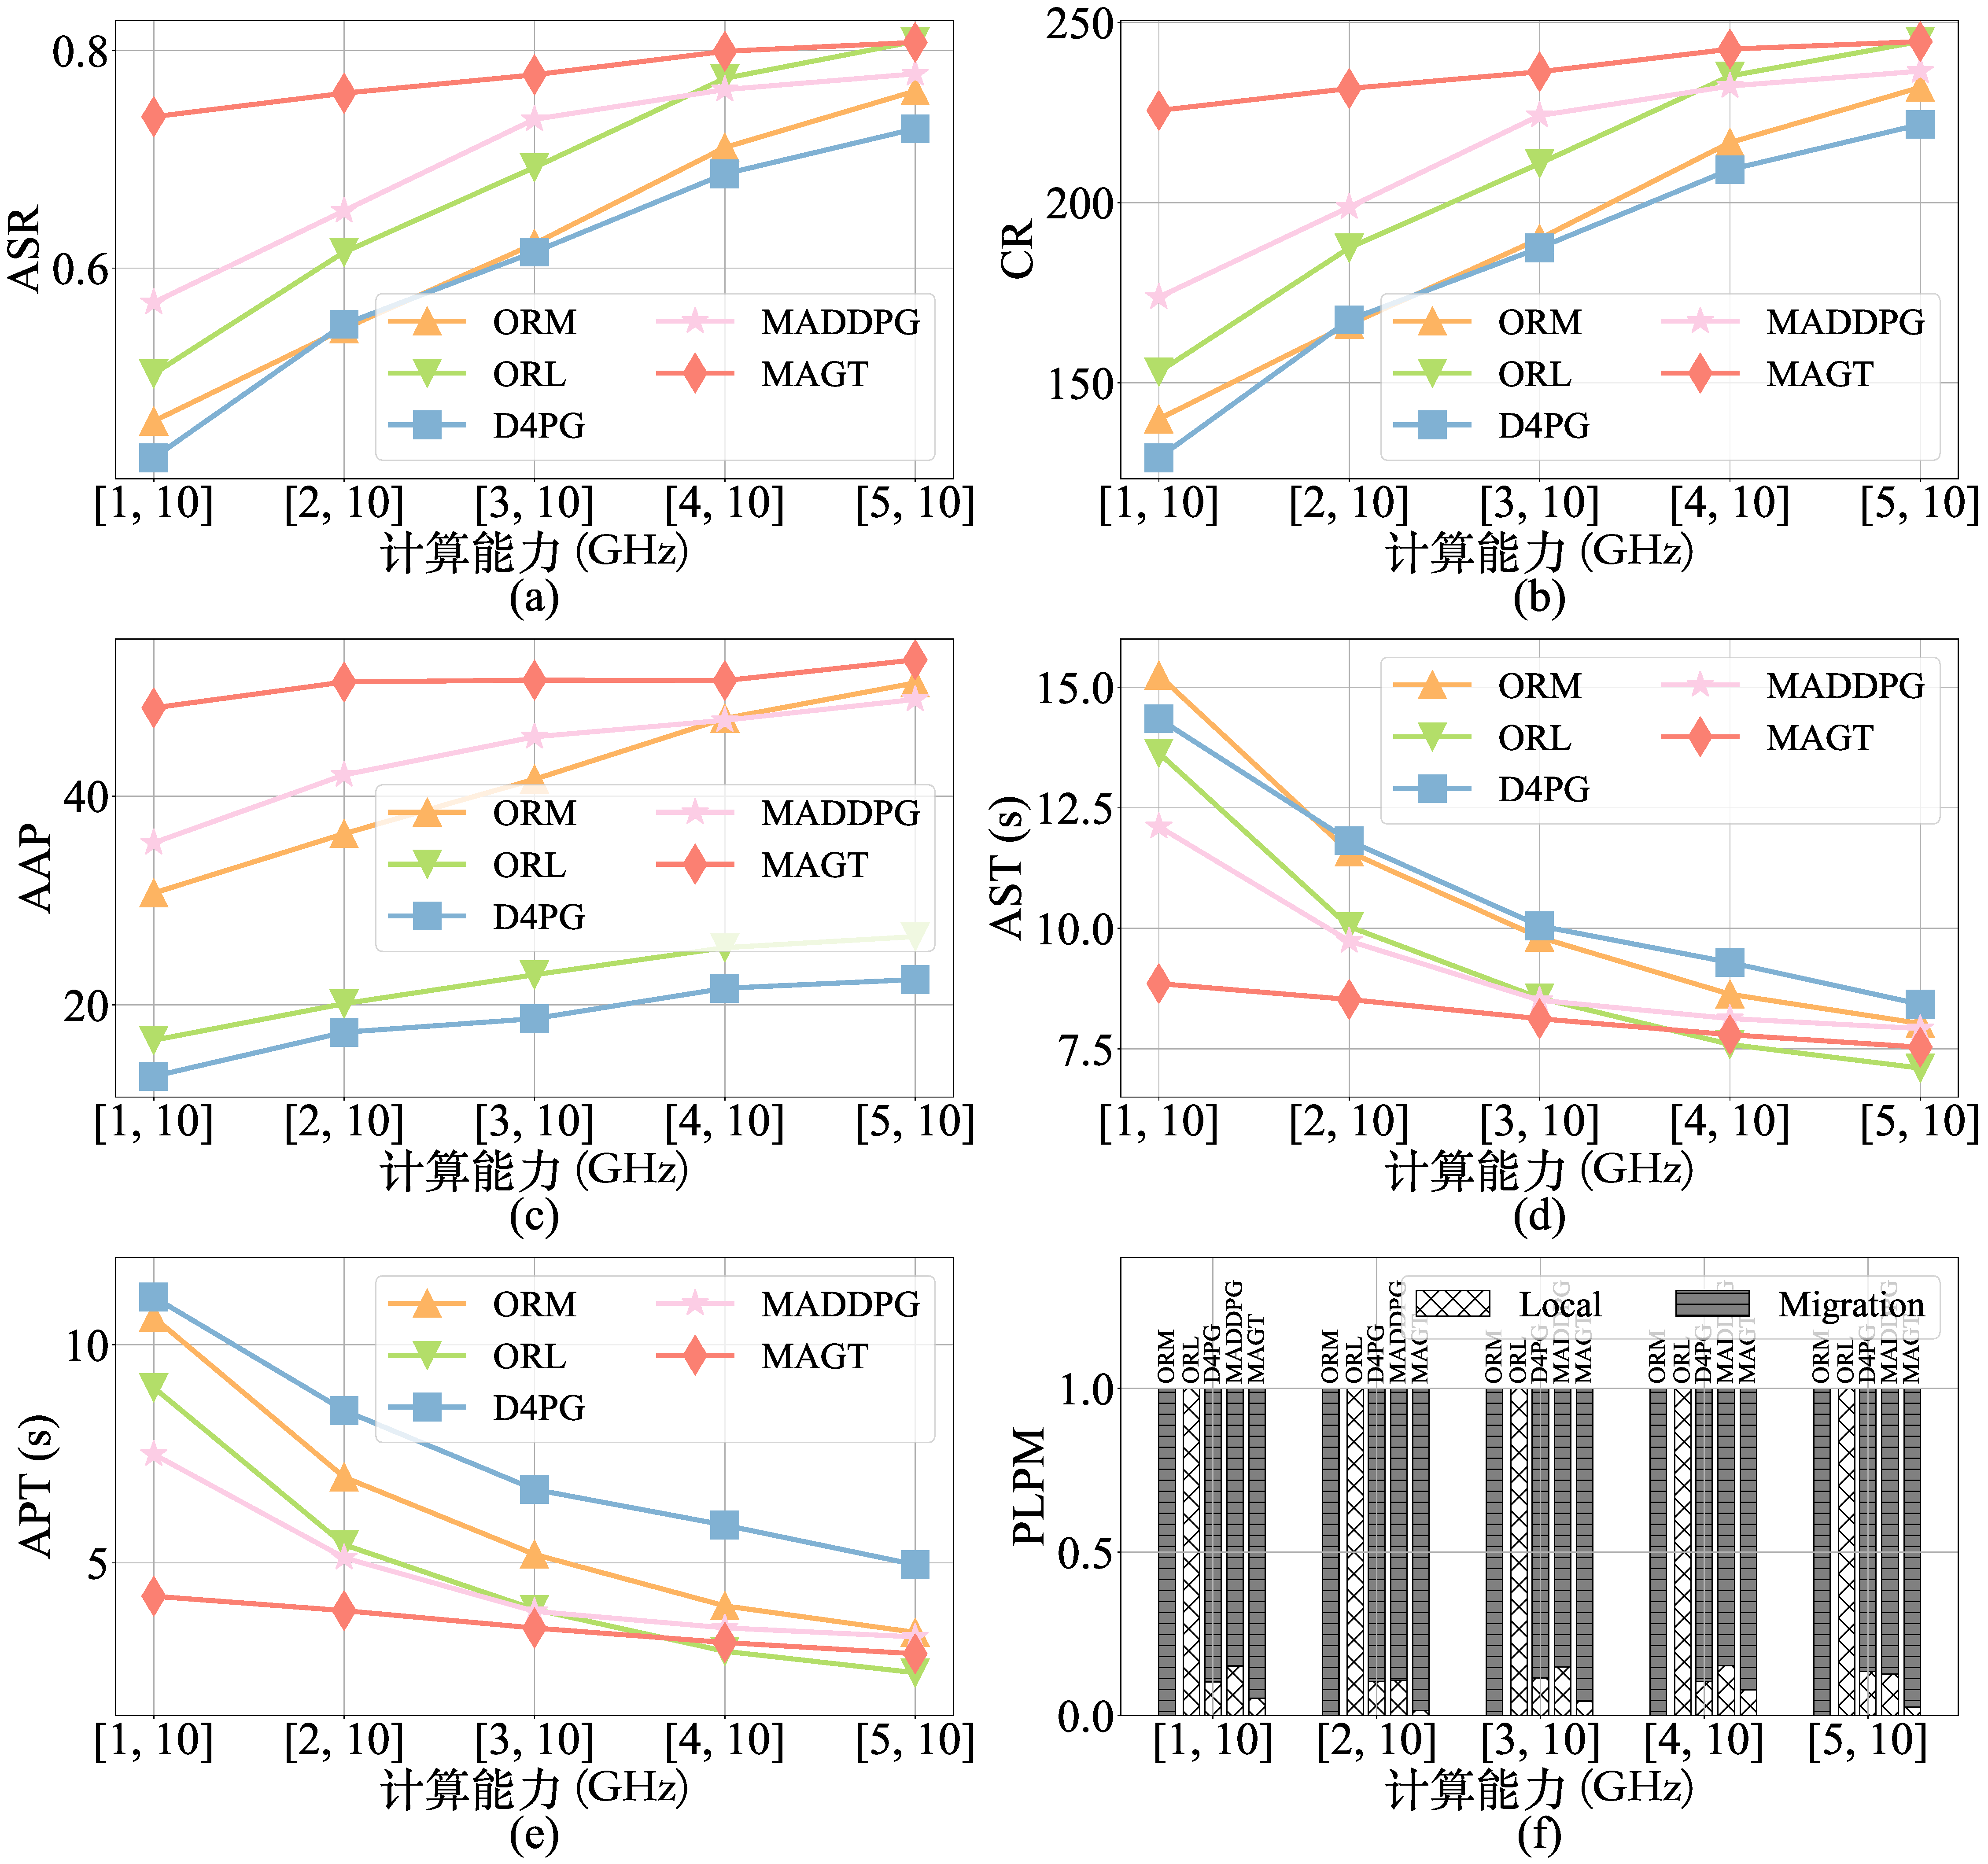
\includegraphics[width=1\columnwidth]{Fig3-6-different-computation-capability.pdf}
  \bicaption[不同边缘计算能力下的性能比较]{不同边缘计算能力下的性能比较。(a)平均服务率(b)累积奖励(c)平均实现势(d)平均服务时间(e)平均处理时间(f)本地处理与迁移的比例}[Performance comparison under different computation capabilities of edge nodes]{Performance comparison under different computation capabilities of edge nodes. (a) Average service ratio (b) Cumulative reward (c) Average achieved potential (d) Average service time (e) Average processing time (f) Proportion of local processing to migration}
  \label{fig 3-6}
\end{figure}

\textbf{3) 边缘节点计算能力的影响:} 图\ref{fig 3-6}比较了边缘节点不同计算能力下的五种算法性能。在本组实验中,边缘节点的计算能力遵循均匀分布,并从$c_e\sim[1, 10]$ GHz增加到$c_e\sim[5, 10]$ GHz,更大计算能力代表可以执行更多的任务。图\ref{fig 3-6}(a)比较了五种算法的ASR。随着计算能力的增加,所有算法的ASR都相应增加。图\ref{fig 3-6}(b) 比较了五种算法的CR。特别地,MAGT实现了最高的CR。图\ref{fig 3-6}(c)比较了五种算法的AAP。正如预期,当计算能力增加时,所有五种算法的性能都会变好。图(d)比较了五种算法的AST。本章注意到,当边缘节点的计算能力比较大时(即$c_e\sim[4,10]$ GHz和$c_e\sim[5,10]$ GHz),ORL的AST低于MAGT。原因是不同边缘节点的计算能力之间的差距变小。因此,当任务在本地执行时,任务的处理时间比卸载到其他边缘节点要短。这可以在图中进一步验证,图中显示了五种算法的APT。本章注意到,当计算能力较大时,ORL的APT是最短的;然而,ORL的ASR比MAGT要小。这是因为在MAGT中,边缘节点之间的通信和计算的合作更加有效。图\ref{fig 3-6}(f)显示了五种算法的PLPM,可以进一步确信这一优势。

\begin{figure}[h]
\centering
  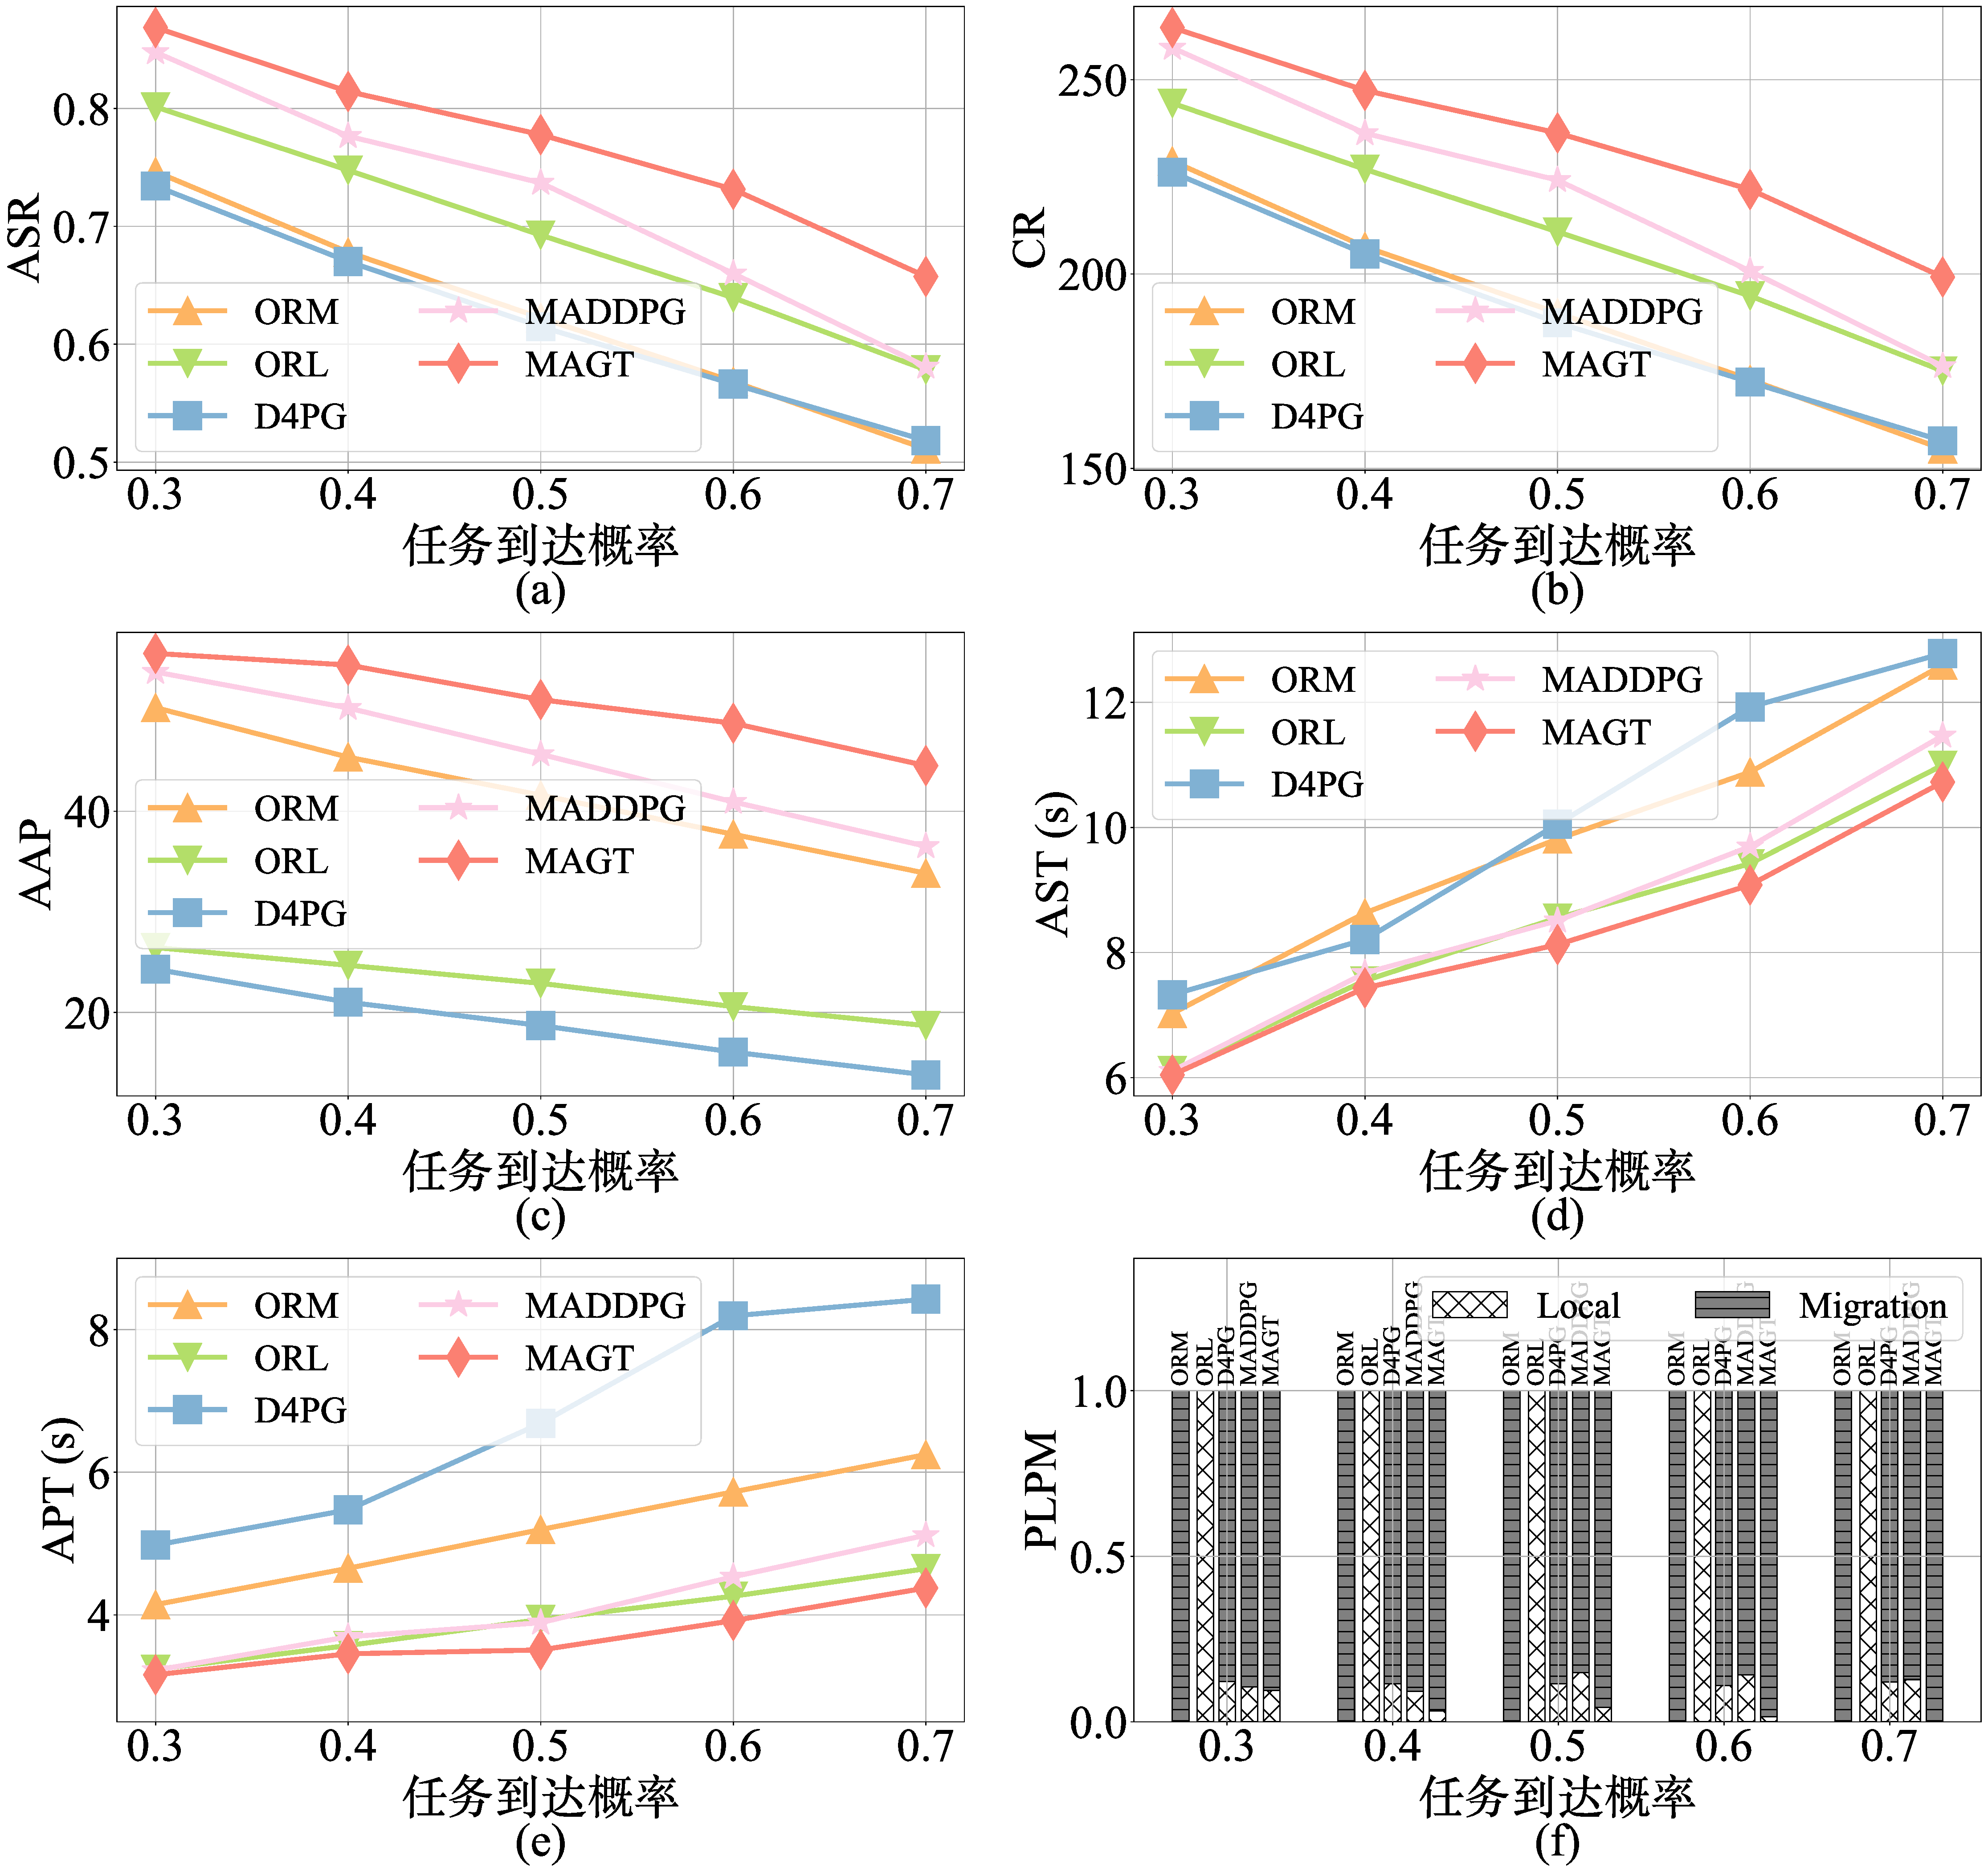
\includegraphics[width=1\columnwidth]{Fig3-7-different-task-arrival-probability.pdf}
  \bicaption[不同任务到达概率下的性能比较]{不同任务到达概率下的性能比较。(a)平均服务率(b)累积奖励(c)平均实现势(d)平均服务时间(e)平均处理时间(f)本地处理与迁移的比例}[Performance comparison under different arrival probabilities of tasks]{Performance comparison under different arrival probabilities of tasks. (a) Average service ratio (b) Cumulative reward (c) Average achieved potential (d) Average service time (e) Average processing time (f) Proportion of local processing to migration}
  \label{fig 3-7}
\end{figure} 

\textbf{4) 任务到达概率的影响:} 图\ref{fig 3-7}比较了不同车辆任务到达概率下的五种算法的性能。在本组实验中,车辆在每个时隙的任务到达概率从$\tau_{v}^{t}=0.3$增加到$\tau_{v}^{t}=0.7$。正如预期,当任务到达概率增加时,五种算法的性能都会变差。图\ref{fig 3-7}(a) 比较了五种算法的ASR,MAGT实现了最高的ASR。图\ref{fig 3-7}(b) and \ref{fig 3-7}(c) 比较五种算法的CR和AAP,显示MAGT在所有情况下都能保持最高的CR和AAP,这表明MAGT通过采用势函数作为边缘节点奖励的优势。图\ref{fig 3-7}(d) 和 图\ref{fig 3-7}(e) 比较五种算法的AST和APT。可以看出,当任务到达概率从0.3增加到0.4时,ORL、MADDPG和MAGT之间的性能差距很小。原因是,当有足够的资源时,算法的调度效果变得不明显。图\ref{fig 3-7}(f) 比较了五种算法的PLPM。当任务到达概率增加时,MAGT中本地处理的任务比例下降。原因是迁移到其他边缘节点的任务更有可能在任务截止时间前得到服务。

\section{本章小结}\label{section 3-6}

本文提出了一个基于NOMA的VEC架构,用于边缘节点之间的合作通信和计算。
在此基础上,通过考虑边缘内和边缘间干扰的建立了V2I传输模型,并通过考虑异构资源和边缘节点间的合作建立了任务卸载模型。
然后,本章提出了CRO问题,其目标为最大化任务服务率。
此外,本章将CRO分解为两个子问题,即任务卸载和资源分配。
任务卸载子问题被建模为一个具有NE存在和收敛性的EPG。
提出了MAGT算法,其中边缘节点作为智能体,在行动空间中决定任务卸载策略以实现NE。
特别地,博弈模型的势函数被作为边缘节点的奖励。
然后,根据基于梯度的迭代方法和KKT条件,提出了解决资源分配问题的最优方案。
最后,本章利用从不同时期提取的真实车辆轨迹建立了仿真模型,并通过综合性能评估证明了所提方案的优越性。
